\chapter{Defining the system}
The definition of the system plays an essential role as it sets the scene for
the whole study. With the general goal of investigating the frictional behvaiour
of a graphene sheet, as we alter it through kirigami cuts and stretch, two
different approaches was considered as sketched in \cref{fig:system_variations}.
One approach is simply to mimic a \acrshort{FFM} type experiment as done in most
other numerical friction studies. In this case, we probe the graphene sheet,
resting on a substrate, with an indenting tip connected to a moving body.
Friction is then measured by making the tip scan across the graphene surface.
This setup allows for a variety of tip shapes and sizes, and alternatively the
tip can be substituted with a flat surface making the setup resemble a
\acrshort{SFA} experiment. It is not obvious how one would achieve the
stretching of the sheet, but a simple solution is to pre-stretch the sheet to a
given amount and then fixating it, by the ends, on the substrate. We are then
able to investigate the frictional behaviour at different amounts of stretching
between simulations. If any interesting behvaiour is found, at a certain stretch
amount, a possible application would call for the attatchment of a pre-stretched
sheet as a surface coating. Another option is to attatch the graphene sheet to
the moving body instead and introduce some sort of nanomachine in the moving
body coupling the normal load with a stretching motion. This gives more
design room to utilize any stretch-related friciton effects that require a
dynamical changing of the stretch amount throughout the loading. While both
methods serve as novel approaches with prospects of providing valuable insight
into a sparsly covered field, we choose the latter option due the increased
application design freedom. Hence, our system of choice
consists of two seperate parts: A 2D graphene sheet and a 3D Silicon ``bulk''
substrate. Note, that we do attempt to model the nanomachine explicitly in this
study, but we will consider the prospects of adding this in
\cref{chap:negative_coef}. 


\begin{figure}[H]
  \centering
  \includegraphics[width=0.8\linewidth]{figures/system/system_variations.png}
  \caption{\hl{TMP} System variations}
  \label{fig:system_variations}
\end{figure}


% By applying a normal force and a tangential force we can investigate the friction behvaiour of the contact interface between the sheet and substrate.

% which interact through \acrshort{LJ} potential modelling a van der Waals force. 

\section{Region definitions}
We subdivide the two main parts of the simmulation, the sheet and the substrate, into specific regions according their functionality in the \acrshort{MD} simmulations. For the sheet, we denote a subsection of the ends, with respect to the sliding direction, as so-called \textit{pull blocks}, which is reserved for the application of normal load, stretching and
dragging of the sheet, and for applying the thermostat. The remaining \textit{inner
sheet} is left for the kirigami cuts and are simulated as an $NVE$ ensemble. The pull blocks are equally split between a thermostat part and a rigid part. The rigid part is however thermolized during the initial relaxtion period but made rigid for the final duration of the simulation. Note that the rigid parts on both sides of the sheet is then considered as a single rigid object even though
they are physically seperated. This means that all force interactions concerning the rigid parts will be applied as a common average making them move in total synchronization. The substrate is equally divided into three parts: The
\textit{upper layers} ($NVE$) responsible for the sheet-substrate interaction, the
\textit{middle layers} being a thermostat ($NVT$), and the \textit{bottom layers} being frozen, made rigid and fixed, in the initial lattice structure to ensure that the substrate stays in place. In \cref{fig:system} the system is displayed
with colors matching the three distinct roles:
\begin{enumerate}
  \item Red: $NVE$ parts which is governing the frictional behaviour of interest.
  \item Green: Thermostats ($NVT$) sourrounding the $NVE$ parts in order to modify the temperature without making disturbing changes to the interaction of the sheet and substrate.
  \item Blue: Parts that are initially or eventually turned in to rigid objects. For the substrate this refers to an addtionally fixation as well.
\end{enumerate}
The full sheet is given a size $\sim 130 \times \SI{163}{\text{Å}}$ while the substrate is scaled accordingly to the sheet which is further specified in \cref{sec:substrate}. For an expected stretch of 200\% the total system size is roughly 55k atoms. The specific distribution is shown in \cref{tab:system_count} along with the spatial x-y-measures in \cref{tab:sheet_dim}.


\begin{figure}[H]
  \centering
  \begin{subfigure}[b]{0.80\textwidth}
      \centering
      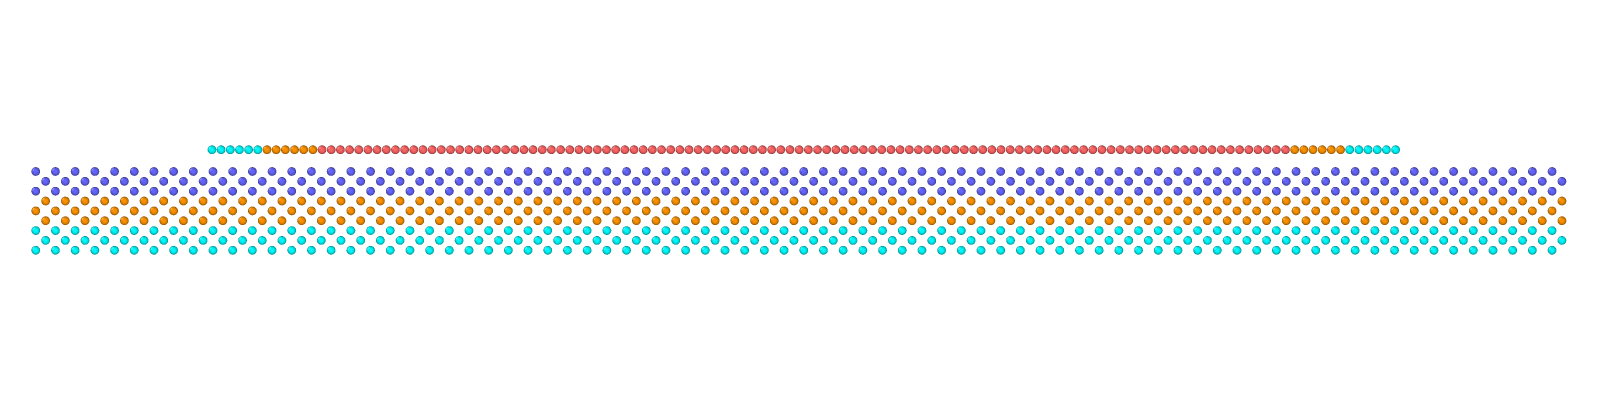
\includegraphics[width=\textwidth]{figures/system/system_sideview.png}
      \caption{Side view showing sheet on top of the substrate.}
      \label{fig:sideview}
  \end{subfigure}
  \hfill
  \begin{subfigure}[b]{0.80\textwidth}
      \centering
      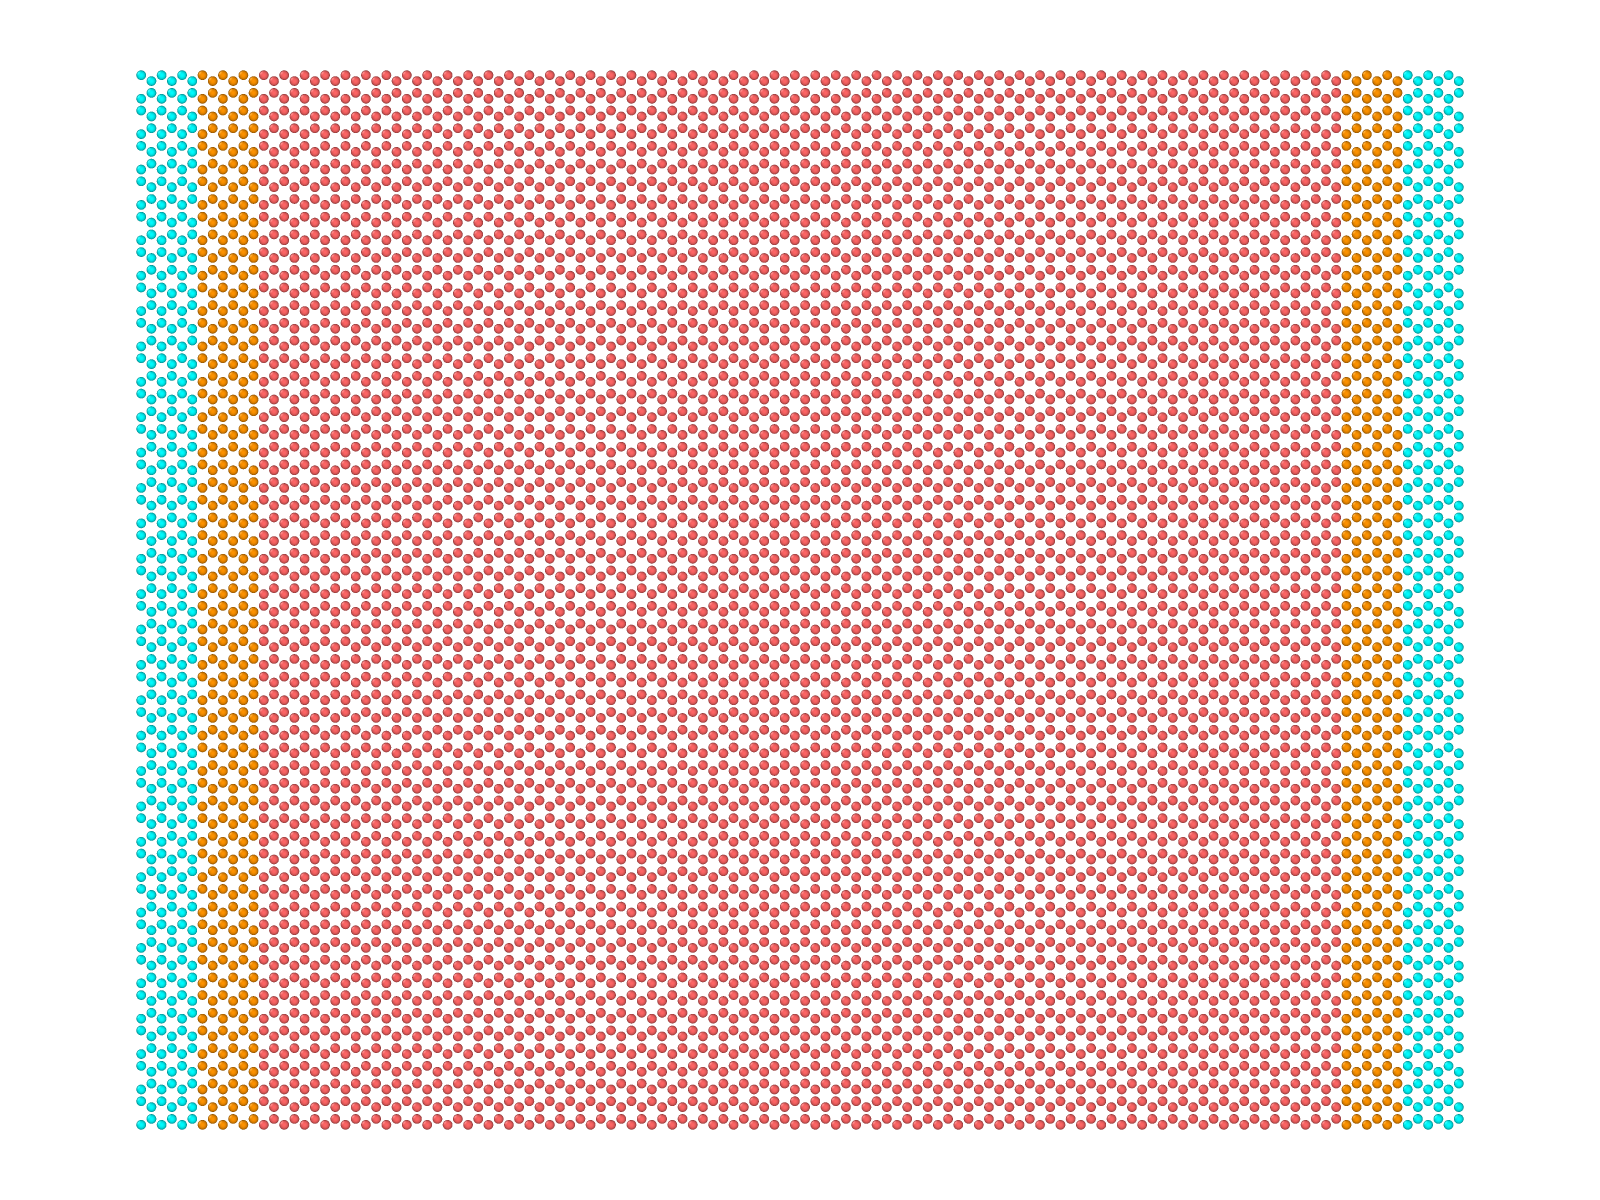
\includegraphics[width=\textwidth]{figures/system/system_topview.png}
      \caption{Top view showing only the sheet.}
      \label{fig:topview}
  \end{subfigure}
  \hfill
     \caption{System configuration colorized to indicate NVE parts (red), thermostat parts (green) and rigid parts (blue).}
     \label{fig:system}
\end{figure}



\begin{table}[H]
  \begin{center}
  \caption{Specification of the spatial size of the system for the x-y-dimensions with a substrate scaled for an expected stretch of 200\%. The first column denotes the size relative to the full sheet size $x_S \times y_S$, while the second column denotes the corresponding length in Å.}
  \label{tab:sheet_dim}
  \begin{tabular}{ | l | r@{}l | r@{}l | c |} \hline
    \textbf{Region} & \multicolumn{2}{c|}{Dim} & \multicolumn{2}{c|}{Dim
    [Å]} & Area [Å$^2$]\\ \hline
  Full sheet & $x_S \: \times \: $ & $y_S$ &  $130.029 \: \times \:$ & $163.219$ Å & $\phantom{2\times} 21,223.203$ \\ \hline
  Inner sheet & $x_S \: \times \:$ & $0.81 \ y_S$ &  $130.029  \: \times \:$ & $132.853$ Å & $\phantom{2\times} 17,274.743$\\ \hline
  Pull blocks & $2 \times x_S \: \times \:$ & $ 0.09 \ y_S$ & $2 \times 130.029  \: \times \: $ & $\phantom{0}15.183$ Å  & $2 \times \phantom{0}1,974.230$ \\ \hline  
  Substrate & $1.16 \ x_S \: \times \:$ & $3.12 \ y_S$ &  $150.709  \: \times \:$ & $509.152$ Å & $\phantom{2\times} 76,733.789$\\ \hline
\end{tabular}
\end{center}
\end{table}



\begin{table}[H]
  \begin{center}
  \caption{Specification of the system size in number of atoms for various system regions. These numbers corresponds with the case of no cuts applied to the sheet and a substrate scaled for the expected stretch of 200 \%.}
  \label{tab:system_count}
  \begin{tabular}{ |c?{0.3mm} c | c | c | c | c | c |} \hline
    \textbf{Region} & \textbf{Total}  & Sub region & Sub total & \textbf{NVE} &
    \textbf{NVT} & \textbf{Rigid} \\ \hline   
    \multirow{2}{*}{Full sheet} & \multirow{2}{*}{7800} & Inner sheet & 6360 & 6360 &
    0 & 0 \\ %\hline
    & & Pull blocks & 1440 & 0 & 720 & 720 \\ \hline   
    \multirow{3}{*}{Substrate} & \multirow{3}{*}{47376} & Upper & 15792 & 15792 &
    0 & 0 \\ %\hline
    & & Middle & 15792 & 0 & 15792 & 0 \\ %\hline
    & & Bottom & 15792 & 0 & 0 & 15792 \\ \Xhline{2\arrayrulewidth}   
    All & 55176 & \multicolumn{2}{r|}{} & 22152 & 16512 & 16512 \\ \hline 
  \end{tabular}
  \end{center}
\end{table}


\section{Numerical procedure}
The numerical procedure related to the measurement of friction can be arranged
into the following steps. Some steps have been given a default duration
denoted in parentheses in units of ps, \num{e-12} seconds.
\begin{enumerate}
  \item \textbf{Relaxation} (15 ps): The sheet and substrate are relaxed for 15 ps after being added in their crystaline form with a seperation distance of 3 Å. The equilibrium seperation distance varies slightly with temperature, but we found this number to be a reasonble middle ground for the temperature range of interest. The sheet is
  constrained under three hard spring forces, all with spring constant $10^5$
  eV/Å$^2$ $\sim$ \num{1.6e6} N/m: One spring attaches the sheet center of mass
  (\acrshort{CM}) to its orginal postion, preventing any drift. The
  remaining two springs are attatched to the pull block ends, to their initial \acrshort{CM} position respectively, to prevent rotation. In principle, it would be sufficient to fixate just one of the ends in order to stop rotation, but we fixate both ends for the sake of symmetry. During the
  relaxtion phase the pull blocks are made rigid with respect to the z-direction
  only (perpendicular to the sheet). That is, all the forces in the z-direction
  is summed up and distributed on the pull blocks as a single external force, while it is free to expand and
  contract in the x-y-plane. This is mainly to ensure that it achieves the
  correct lattice spacing according to the temperature of the system. For the following phases the rigid parts of the pull block is in fact rigid with
  respect to all directions. The spring forces are terminated after the relaxtion phase. 
  \item \textbf{Stretch}: The sheet is stretched by seperating the two opposing rigid parts of the pullblock at constant velocity until the desired stretch amount is met. The duration of this phase is thus governed by the  \textit{stretch speed} and \textit{stretch amount} parameters. 
  \item \textbf{Pause} (5 ps): The sheet is relaxed for 5 ps to ensure that the sheet is stable and equilibrized after the applied stretch deformation. 
  \item \textbf{Normal load} (5 ps): The normal load is applied to the rigid
  parts of the pull blocks. Initially a viscous damping force, $F = -\gamma \vec{v}$, is added to the sheet to resist the rapid acceleraction of the sheet and prevent a hard impact between the sheet and substrate. The damping coefficient is set to $\gamma = \SI{8e-4}{nN/(m/s)}$ and terminated after 0.5 ps which was found to be suitable for the extreme load cases of our intended range. The remaining 4.5 ps is simply devoted for further relaxation. 
  \item \textbf{Sliding}: A virtuel atom is introduced into the simulation which
  exclusively interacts with the rigid parts of the pull blocks through a spring force
  with variable spring constant $K$ in the x-y-plane. The z-direction is not
  affected by the spring force and is purely governed by the balancing forces of the normal load and the normal response from the sheet-substrate interaction. The
  virtual atom is immediately given a constant velocity, in accordance to
  the \textit{sliding speed} parameter, which make the sliding force increase quadratically, $F_{\textit{slide}} \propto K(v_{\text{slide}}t)^2$, with sliding speed. An infinite sprig constant can also be enforced for which the spring is omitted and the pull blocks are moved rigidly with a constant speed according to the sliding speed.
\end{enumerate}
In order to prevent rupturing, or detachment, of the sheet, we monitor the nearest neighbours for each atom throughout the simularion. At the initial timestep the three nearest neighbours, sitting at a distance 1.42 Å, of all graphene atoms is recorded. If any of these nearest neighbours exceeds a threshold distance of 4 Å, indicating a bond breakage, this is marked as a rupture and we halt the simulation early. Thus, we ensure that no wear is taking place for the sheet. The substrate was proven to be way more resistant to wear, and by running a few test simulations of high load and sliding speed we confirmed visually that no wear is accouring.

\section{Creating the substrate}\label{sec:substrate}
The substrate is created as a rectangular slab of Silicon (Si). We create the
initial configuration according to its crystaline structure given as a diamond
cubic crystal with a lattice parameter $a_{\text{Si}} = 5.43$ Å. The default
substrate thickness is choosen such that 9 layers of atoms appear (2 unit cells)
corresponing to a thickness of 10.86 Å. The x-y dimensions is choosen to match the dimensions. That is, we define a margin between the
sheet edge and the substrate edge for the x- and y-direction respectively. Since
we use periodic boundary conditions a too small margin would result in the sheet
edges interacting with themselves through the boundary. The absolute lower limit
for the margin choice is thus half the cut-off distance for the Tersoff potential,
governing the graphene sheet interaction, at $R + D = 2.1$ Å. However, due to
fluctuations in the sheet we cannot set the margin to close to that limit.
Additionally, we must take into account the buckling of the sheet as it is
stretched, which might induce an expansion in the x-direction for certain
configurations. We choose a x-margin of 20 Å which provides $2\cdot
\SI{20}{\text{Å}} - \SI{2.1}{\text{Å}} = \SI{37.9}{\text{Å}}$ of additional
spacing with respect to the absolute lower limit. By looking over the simulation
result visually we confirm that this leaves more than enough room in the cases
of extreme buckling. For the y-direction the rigid parts of the pull-blocks
moves a certain distance based on the stretch value exclusively, and we define
the y-margin based on the remaining distance to the edge after stretching.
However, as the sheet travels through the periodic boundaries in the y-direction
when sliding, we want to add some additional spacing through the y-margin in
order to let the substrate surface relax before interacting with the sheet a
second time. We choose a y-margin of 15 Å for which the preferred sliding speed of
$\SI{20}{m/s} = \SI{2}{\text{Å}/ps}$ gives \SI{15}{ps} of relaxtion time between encounters with the sheet, similar to the inital relaxtion time. 


\section{Creating the sheet}
% \subsection{Graphene}
% (https://community.wvu.edu/~miholcomb/graphene.pdf)
% https://www.physics-in-a-nutshell.com/article/4/lattice-basis-and-crystal

The sheet is created by the 2D material known as graphene which consist of a single layer of carbon atom arramged in hexagonal lattice structure. The bulk version of this material is called graphite and simple referes to the merged structure of multiple graphene layers. We can describe the 2D crystal structure in terms of its primitive lattice vectors $\vec{a_1}$ and $\vec{a_2}$ and a basis. The basis describes the .. part of the crystal and we populate each lattice site by the given basis and translate it to fill the whole plane by any linear combination of the lattice vectors 
\begin{align*}
  \vec{T}_{mn} = m\vec{a_1} + n\vec{a_2}, \qquad m,n \in \mathbb{N}.
\end{align*}
For graphene, we have the primitive lattice vectors 
\begin{align*}
  \vec{a_1} = a \left(\frac{\sqrt{3}}{2}, -\frac{1}{2}\right), \qquad \vec{a_2} = a \left(\frac{\sqrt{3}}{2}, \frac{1}{2}\right), \qquad |\vec{a_1}| = |\vec{a_2}| = 2.46 \ \text{Å}.
\end{align*}
Notice that we deliberately excluded the third coordinate as we only consider a
single graphene and thus we do not have to consider the stacking structure of 3D graphite. The basis consist of two carbon atoms given as 
\begin{align*}
  \Big\{\Big(0,0\Big), \frac{a}{2}\Big(\frac{1}{\sqrt{3}}, 1 \Big) \Big\}
\end{align*}
The crystal structure is visualized in \cref{fig:graphene_crystal}. It turns out that the spacing between atoms is equal for all pairs of atoms with an interatomic distance
\begin{align*}
  \left|\left|\frac{a}{2}\Big(\frac{1}{\sqrt{3}}, 1 \Big)\right|\right| \approx 1.42 \ \text{Å}.
\end{align*}


\begin{figure}[H]
  \centering
  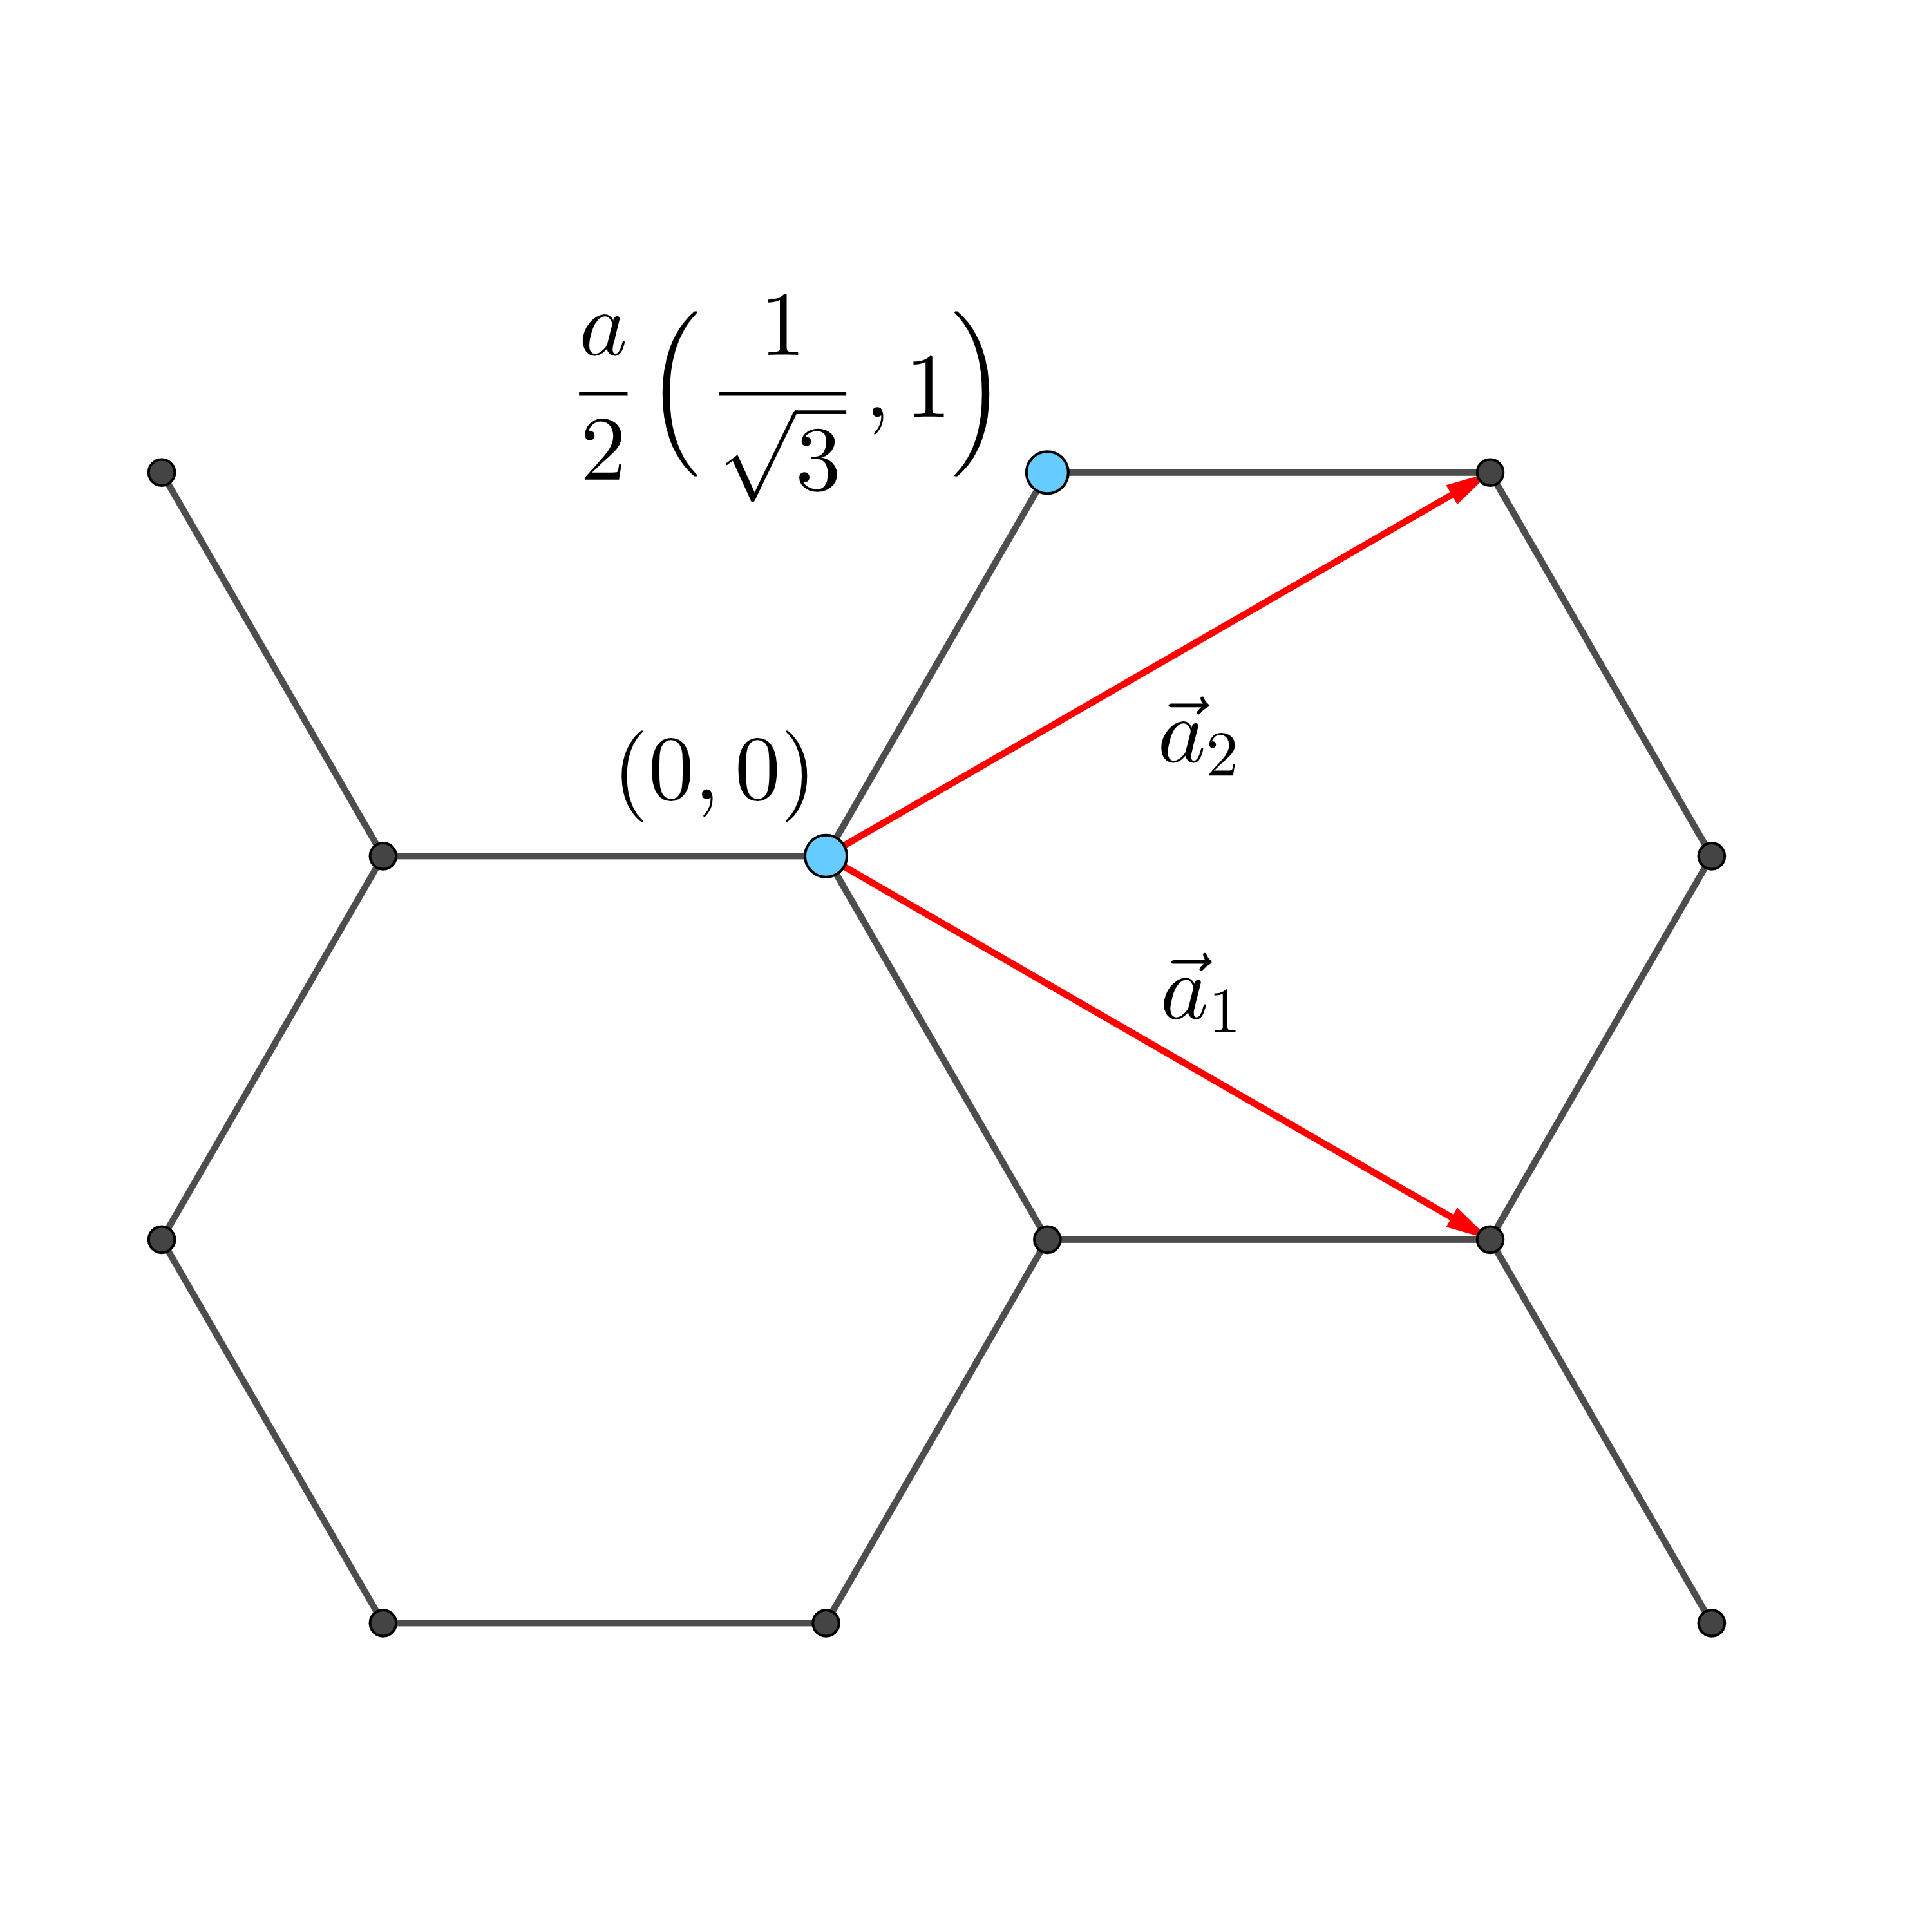
\includegraphics[width=0.3\linewidth]{figures/system/crystal.png}
  \caption{Graphene crystal structure with basis.}
  \label{fig:graphene_crystal}
\end{figure}



\subsection{Indexing}
In order to define the cut patterns applied to the graphene sheet we need to
define an indexing system. We must ensure that this gives an unique description
of the atoms as we eventually want to pass a binary matrix, containing 0 for
removed atoms and 1 for present atoms, that uniquely describes the sheet. We do
this by letting the x-coordinate allign with the so-called \textit{armchair}
direction of the sheet and making the y-coordinate increment along the
so-called \textit{zigzag} direction. Notice that the x-coordinate will point
point to \textit{zigzag} chains of atoms for which the starting point, at $y = 0$ is not evenly spacedd as illustrated in figure \cref{fig:atom_indexing}. Other solutions
might naturally invole the lattice vectors, but since these are used to
translate between similar basis atoms it introduces an unfortunate duality as
one would then need to include the basis atom of choice into the indexing system
as well. Additionally, we want an indexing system which conserves the relative
physical position of neighbours. That is, atom $(i, j)$ should be in the
proximity of $\{(i+1, j), (i-1, j), (i, j+1), (i, j-1)\}$. However, due to the hexagonal structure of the lattice, only three said neighbour indexes will be actual nearest neighbours in the lattice. While $(i, j\pm 1)$ is always a nearest neighbour, the index of the nearest neighbour in the x-direction oscillate for each incrementing of x- or y-coordinate. That is, the nearest neighbours (\acrshort{NN}) is decided as
\begin{equation}
  \begin{aligned}
    (i + j) \ \text{is even} &\rightarrow \text{\acrshort{NN}} = \{(i-1, j), (i, j+1), (i, j-1)\}, \\
    (i + j) \ \text{is odd} &\rightarrow \text{\acrshort{NN}} = \{(i+1, j), (i, j+1), (i, j-1)\}.
  \end{aligned}
  \label{eq:atom_neigh_idx}
\end{equation}
By consulting \cref{fig:atom_indexing} we can verify this visually, and it basically comes down to the fact whether the atom is oriented to the right or theleft side in the zigzag chain.

\begin{figure}[H]
  \centering
  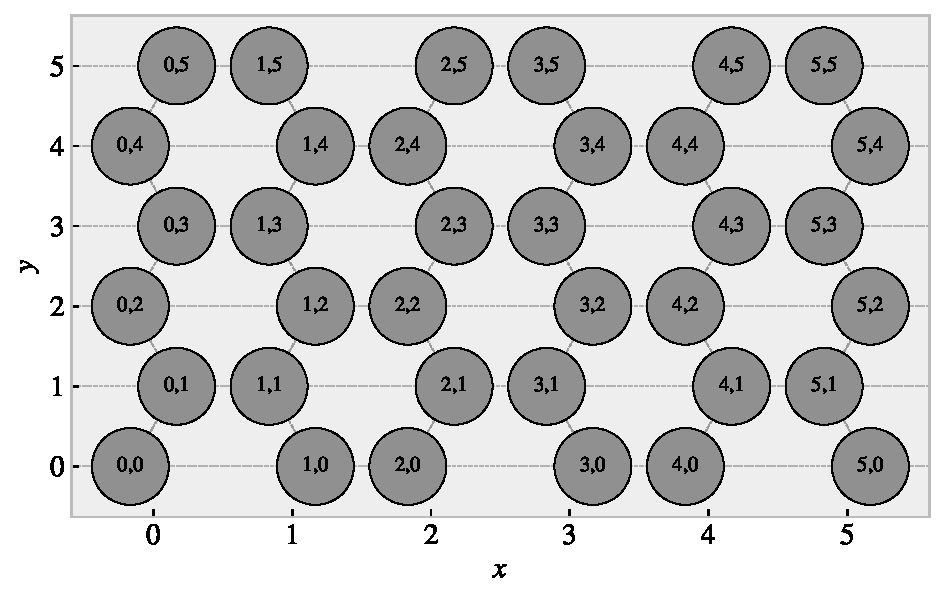
\includegraphics[width=0.7\linewidth]{figures/system/atom_indexing.pdf}
  \caption{Graphene atom indexing}
  \label{fig:atom_indexing}
\end{figure}



\subsection{Removing atoms}
As a means to ease the formulation of the cut patterns we introduce the \textit{center element} placed in each gap of the hexagonal honeycomb structure as shown in figure \cref{fig:center_indexing}. These are not populated by any atoms but will serve as a temporary reference for the algorithmic approaches of defining a cut pattern.

\begin{figure}[H]
  \centering
  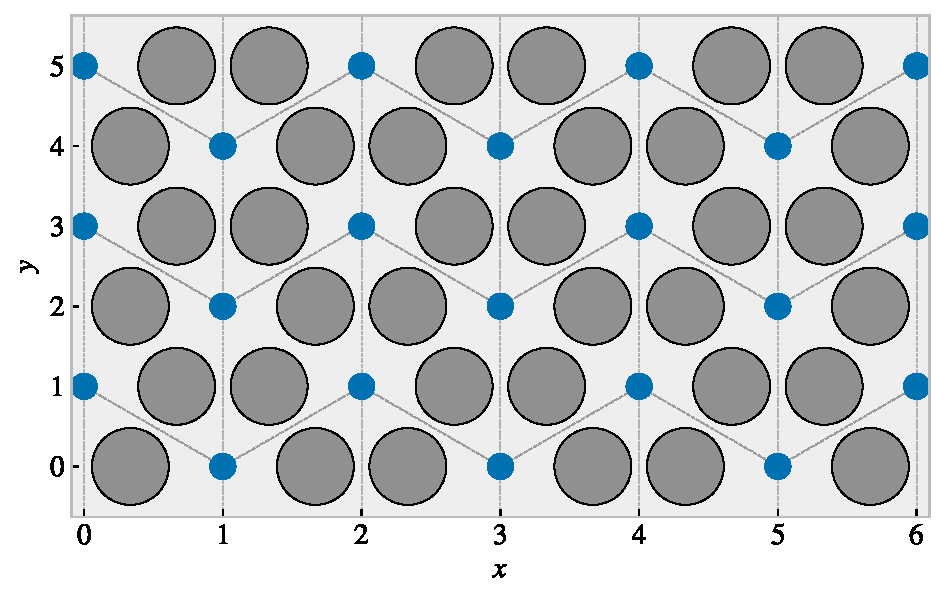
\includegraphics[width=0.7\linewidth]{figures/system/center_indexing.pdf}
  \caption{Graphene center indexing}
  \label{fig:center_indexing}
\end{figure}

Similar to the case of the atom indexing, the nearest neighbours center elements alternate with position, this time only along the x-coordinate index. Each center element has six nearest neighbours, in clockwise
direction we can denote them: ``up'', ``upper right'', ``lower right'',
``down'', ``lower left'', ``upper left''. The ``up'' and ``down'' is always
accesed as $(i,j\pm 1)$, but for even $i$ the $(i+1,j)$ index corresponds to the
``lower right'' neighbour while for odd $i$ this corresponds to the ``upper
right'' neighbour. This shifting applies for all left or right oriented neighbours and the full neighbour list is illustrated in \cref{fig:center_directions}. 


\begin{figure}[H]
  \centering
  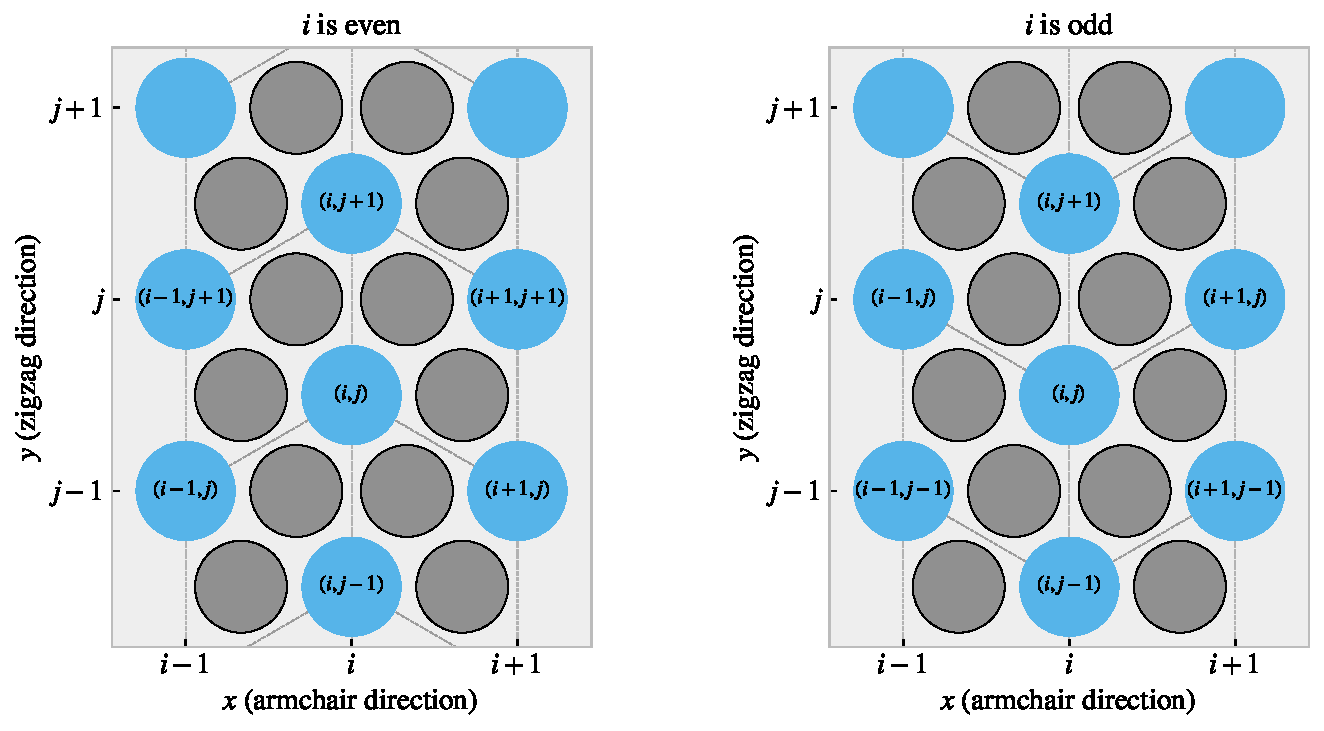
\includegraphics[width=0.7\linewidth]{figures/system/center_directions.pdf}
  \caption{Graphene center elements directions}
  \label{fig:center_directions}
\end{figure}

We define a cut pattern by connecting center elements into connected paths. As
we walk from center element to center element we remove atoms according to one of two rules 
\begin{enumerate}
  \item Remove intersection atoms: We remove the pair of atoms placed directly
  in the path we are walking. That is, when jumping to the ``up'' center
  element we remove the two upper atoms located in the local hexagon of atoms.
  This method is sensitive to the order of the center elements in the path. 
  \item Remove all surrounding atoms: We simply remove all atoms in the local
  hexagon surrounding each center element. This method is indepdent of the
  ordering of center elements in the path.
\end{enumerate}
We notice that removing atoms using either of these rules will not garuantee an injective, one to one, mapping. The first rule, being path dependent, will more often result in a unique result. However, for both methods it is possible to construct two different paths leading to the same cut pattern as shown in the following example:
\begin{align*}
  \text{Path 1:} \quad (i, j) &\rightarrow \underbrace{(i+1,j+1)}_{\text{upper right}} \rightarrow \underbrace{(i, j+1)}_{\text{up}} \rightarrow \underbrace{(i+1, j+2)}_{\text{upper right + up}} \rightarrow \underbrace{(i+1, j+1)}_{\text{upper right}} \\
  \text{Path 2:} \quad (i, j) &\rightarrow \underbrace{(i+1,j+1)}_{\text{upper right}} \rightarrow \underbrace{(i+1, j+2)}_{\text{upper right + up}} \rightarrow \underbrace{(i, j+1)}_{\text{up}}
\end{align*}
\hl{Illustrate the example path, because I think it is otherwise impossible to follow.}

For the second rule it is even more abovious that different paths can result in the same final pattern. For instance, if we incircle a center element completely there will be no surrounding atoms left to delete when jumping to that center element. This highlights the importance of defining the atom based indexing system will yield an injective mapping for the binary cut matrix. However, using the center elements for reference makes the following definitions of the cut patterns a lot easier to design as we always can always go in the same six directions as opposed to the atom indexing system which have alternating directions for its neighbours. 

\section{Kirigami patterns}
We propose a series of kirigami inspired cut patterns for the altering of the graphene sheet. We seek inspiration from macroscale patterns that showcases a considerable amount of out of plane buckling when stretched. We choose to imitate two different designs: 1) An alternating repeating series of perpendicular cuts as shown in \cref{fig:kirigami_inspiration_a} popularly used in studies of morphable metematerials \cite{new_pop_up}. This patteren produce surface buckling with a tetrahedron (three sided pyramid) shape when stretched. 2) A more intricate pattern shown in \cref{fig:kirigami_inspiration_b} which is used commercially by Scotch\textsuperscript{TM} Cushion Lock\textsuperscript{TM} \cite{cushion_wrap} as protective wrap for items during shipping. This pattern buckles into a hexagoal honeycomb structure when stretched. In addition to the modeling of the so-called \textit{Tetrahedron} and \textit{Honeycomb} patterns we also create a series of random walk cut patterns.

\begin{figure}[H]
  \centering
  \begin{subfigure}[t]{0.48\textwidth}
      \centering
      \includegraphics[width=\textwidth]{figures/system/pop_up_inspiration.png}
      \caption{}
      \label{fig:kirigami_inspiration_a}
    \end{subfigure}
    \hfill
    \begin{subfigure}[t]{0.48\textwidth}
      \centering
      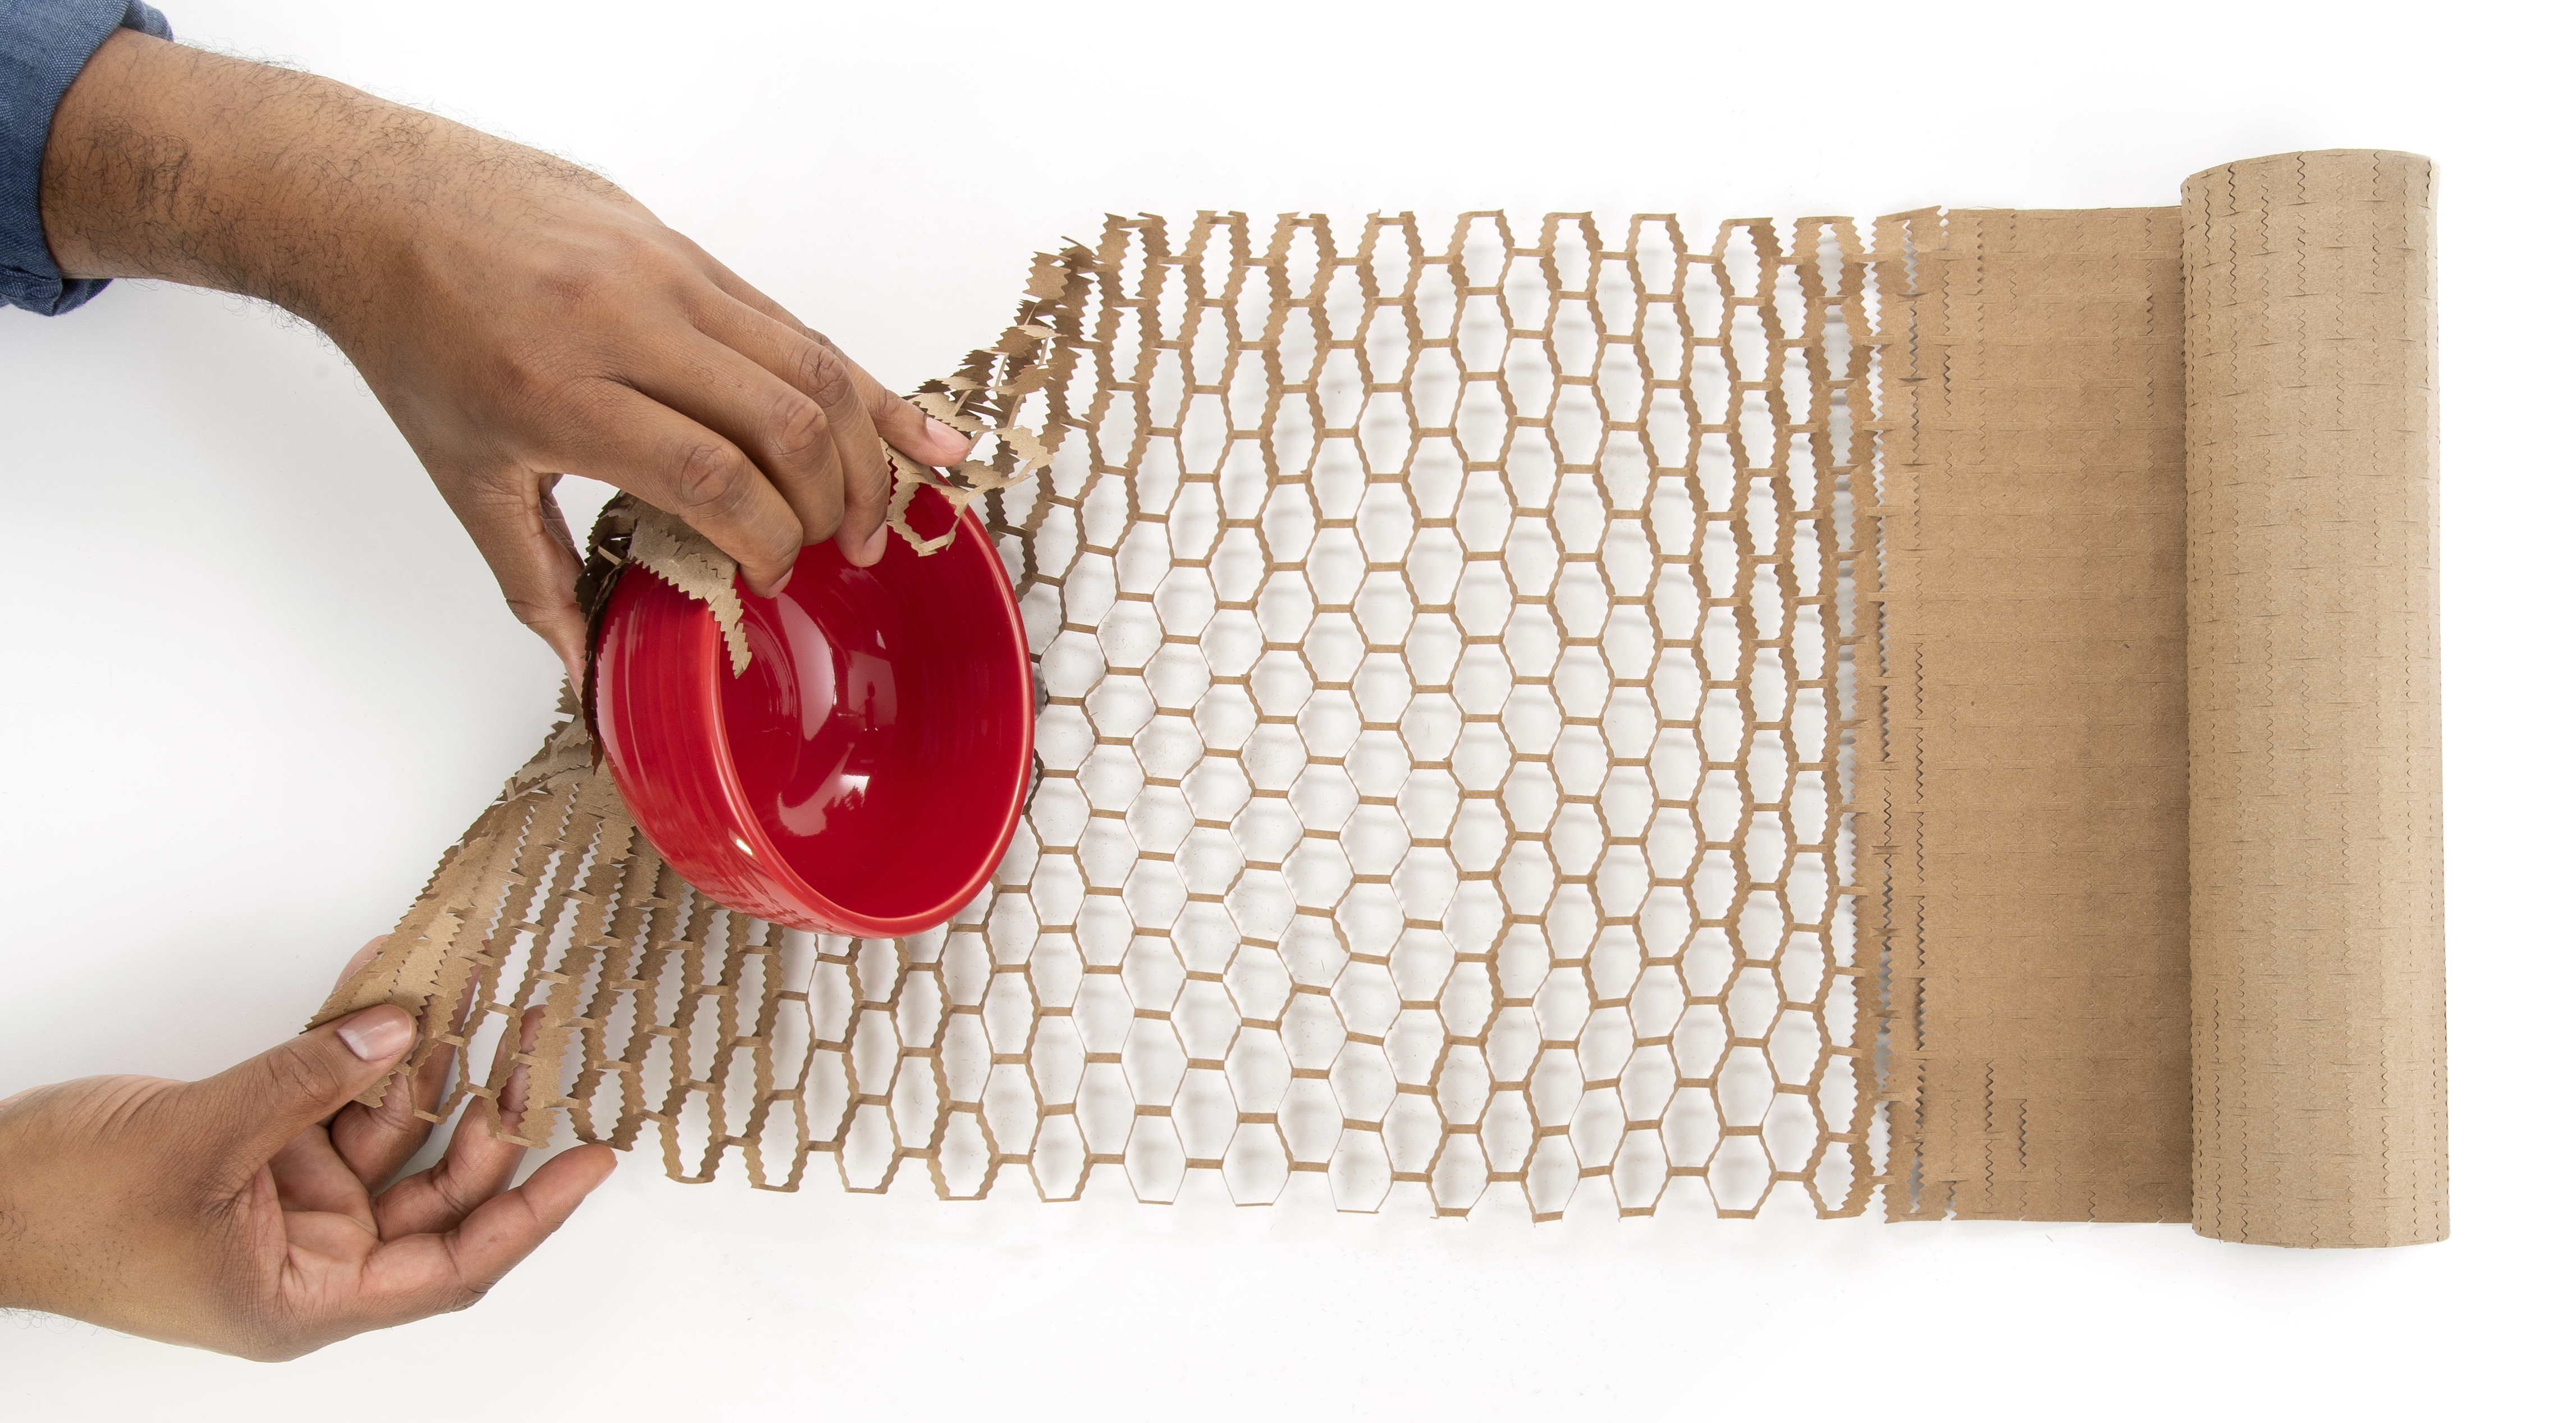
\includegraphics[width=\textwidth]{figures/system/honeycomb_inspiration.jpg}
      \caption{}
      \label{fig:kirigami_inspiration_b}
  \end{subfigure}
  \hfill
     \caption{Macroscale kirigami cut patterns used as inspiraton for the nanoscale implementation. (a) Tetrahedron: Alternating perpendicular cuts producing a tetrahedron shaped surface buckling when stretched \cite{new_pop_up}. (b) Honeycomb: Scotch\textsuperscript{TM} Cushion Lock\textsuperscript{TM} \cite{cushion_wrap} producing a honeycomb shaped surface buckling when stretched.}
     \label{fig:kirigami_inspiration}
\end{figure}

\subsection{Tetrahedron}
The \textit{Tetrahedron} pattern is defined in terms of center elements for
which all atoms sourrounding a given center element are removed. The pattern is
characterized by two straight cuts, denoted line 1 and line 2, arranged
perpendicular to each other. This is done in such a way such that one line aligns with the center of the
other line and with a given spacing in between. This is illustarted in \cref{fig:pop_up}. In order to achieve
perpendicular cuts we cannot rely purely on the six principal directions
corresponding to the center element neighbours which is spaced by 60$^\circ$.
We let line 1 run along the center elemnts in the direction of the
``upper right'' (and ``lower left'') center elements  while line 2 goes in the
direction between the ``down'' and ``lower right'' (``up'' and ``upper left'') center elements, corresponding to the direction $(1/\sqrt{3}, -1)$. We define variations of the pattern by the number of center elements $L_1$ and $L_2$ in line 1 and 2 respectively, together with the spacing between the lines $d$, as the tuple $(L_1, L_2, d)$. The pattern is constructed by translating the two lines to the whole sheet according to the spacing. Due to the alignment criterias of having one line point to the center of the other line we can only have odd line length. Furthermore, in order to ensure that each center element is translated to an $i$-index of similar odd or eveness, we must in practice require that $|L_2 - L_1| = 2, 6, 10, \ldots \ $. In \cref{fig:pop_up} we see a visual representation of the pattern components for the $(7, 5, 2)$ patteren. 


\begin{figure}[H]
  \centering
  \begin{subfigure}[t]{0.48\textwidth}
      \centering
      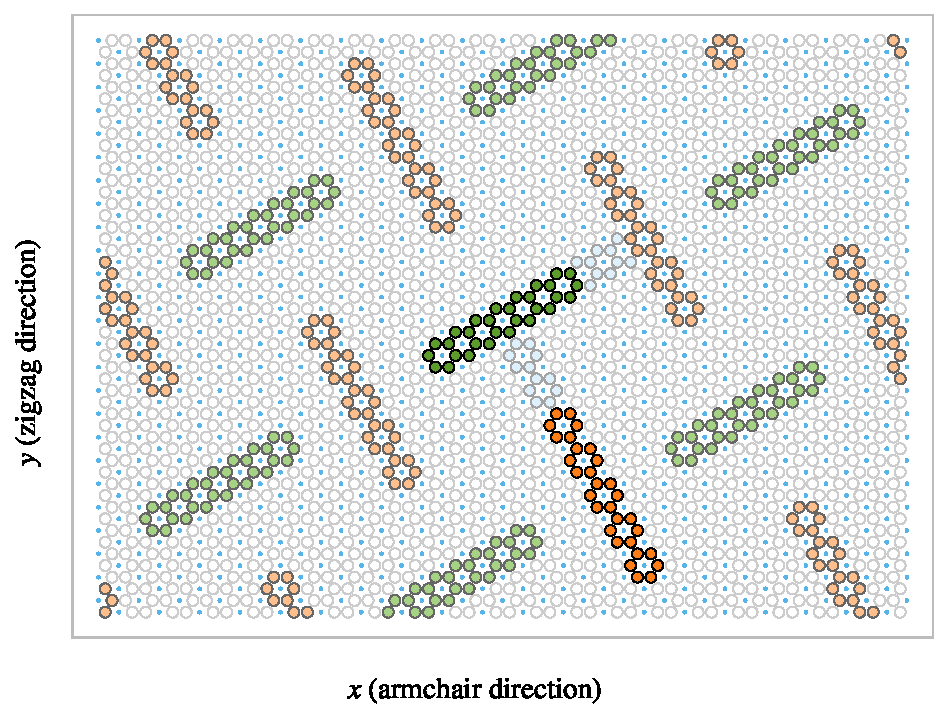
\includegraphics[width=\textwidth]{figures/system/pop_up_inverse.pdf}
      \caption{}
      \label{fig:pop_up_a}
    \end{subfigure}
    \hfill
    \begin{subfigure}[t]{0.48\textwidth}
      \centering
      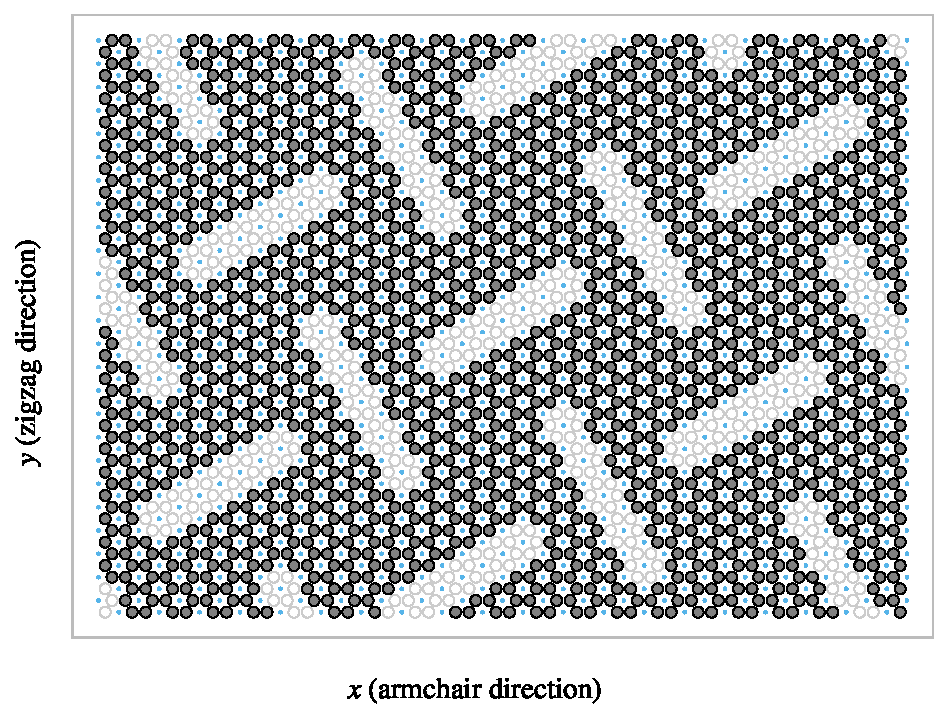
\includegraphics[width=\textwidth]{figures/system/pop_up_pattern.pdf}
      \caption{}
      \label{fig:pop_up_b}
  \end{subfigure}
  \hfill
     \caption{Visual representation of the tetrahedron pattern consisting of two perpendicular lines, line 1 and line 2, of length $L_1$ and $L_2$ respectively with spacing $d$. This example used $(L_1, L_2, d) = (7, 5, 2)$. $(a)$ Highlight of the atoms removed. Line 1 is shown in green and line 2 in orange, with lighter colors for the translated variations, and the spacing is shown in light blue. $(b)$ The sheet after applying the cut pattern where the grey circles denote atoms and the transparent white denotes removed atoms. The small blue circles show the center elements for reference. \hl{Sheet size used in example}}
     \label{fig:pop_up}
\end{figure}

In addition to the three parameters $L_1, L_2, d$, the pattern is also anchored to a reference point which describes the position of line 1 and 2 before translating to the whole sheet. Due to the repeating structure of the pattern there exist a small finite number of unique reference positions. For the pattern $(7, 5, 2)$ used as an example in \cref{fig:pop_up}, there are 140 \footnote{The general formula for this number is rather complicated in comparision to the importance in this context. Thus, we exclude the formula for this calculation as the derivation is rather handwavy executed, but the number stated here is numerically backed for this specific parameter set.} unique reference points. Some additional variation of the pattern is showcased in \cref{fig:pop_up_flavors} all with a reference position in the center of the sheet. Note that a smaller sheet size is used in both \cref{fig:pop_up} and \cref{fig:pop_up_flavors} for illustrative purposes.

\begin{figure}[H]
  \centering
  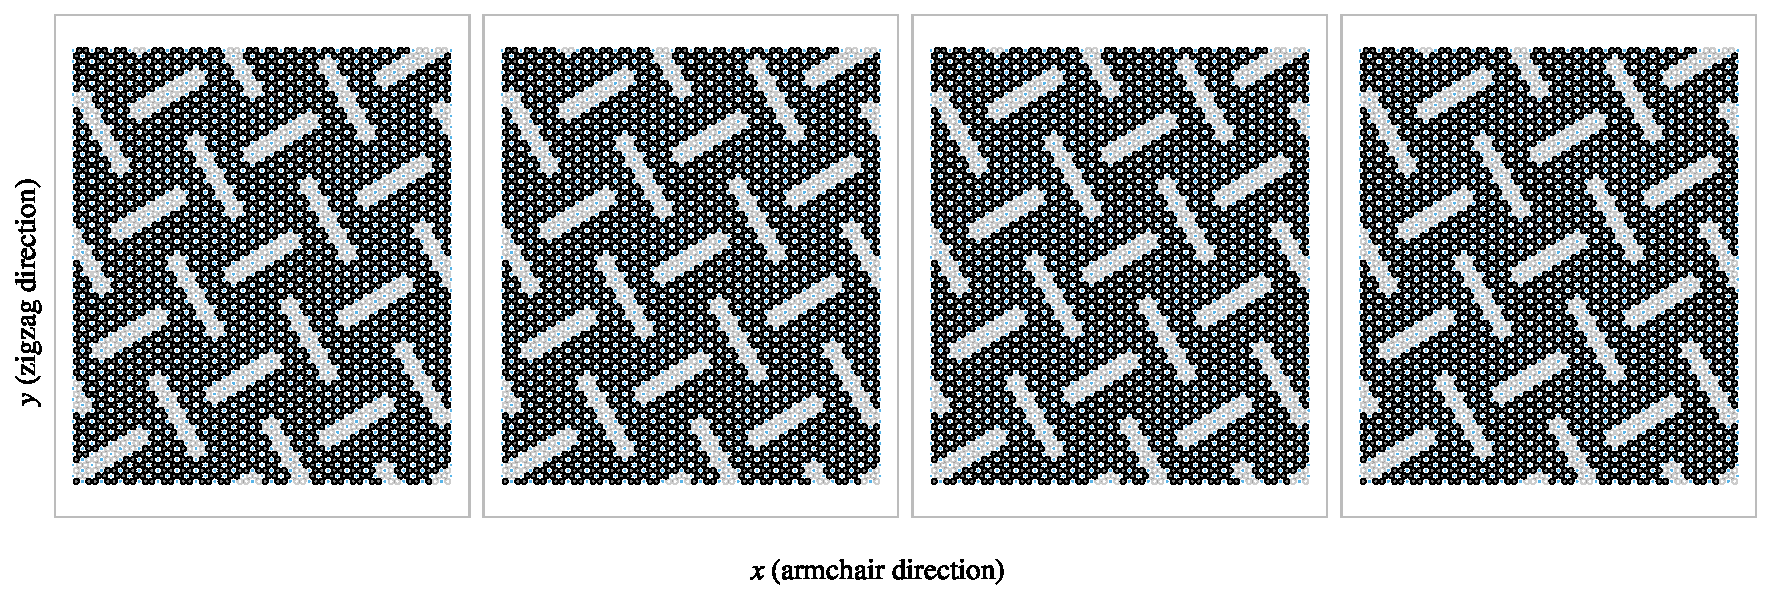
\includegraphics[width=\linewidth]{figures/system/pop_up_flavors.pdf}
  \caption{\hl{Sheet size used in example}}
  \label{fig:pop_up_flavors}
\end{figure}



\subsection{Honeycomb}
The \textit{Honeycomb} pattern is defined, similarly to the Tetrahedron pattern,
in terms of the center elements for which all sourrounding atoms are removed. The Honeycomb pattern is build from a repeating series of
cuts remniscient of the roman numeral one rotated by 90$^{\circ}$
(\rotatebox[origin=c]{90}{\MakeUppercase{\romannumeral 1}}). For a given spacing these are put next to each other in the x-direction, \rotatebox[origin=c]{90}{\MakeUppercase{\romannumeral 1}}
\rotatebox[origin=c]{90}{\MakeUppercase{\romannumeral 1}}
\rotatebox[origin=c]{90}{\MakeUppercase{\romannumeral 1}}, to achieve a row
where only a thin \textit{bridge} in between is left to connect the sheet vertically in the y-direction. By placing multiple rows along the y-direction with alternating x-offsett we get the class of honeycomb patterns as visualized in \cref{fig:honeycomb}. The pattern
is described in terms of the parameters: (x-width, y-width, bridge thickness,
bridge length) which is annotated in \cref{fig:honeycomb_a} with the parameters (2, 2, 1, 5) used as an example. Some additional variations of the pattern class is showcased in \cref{fig:honeycomb_flavors}.


\begin{figure}[H]
  \centering
  \begin{subfigure}[t]{0.48\textwidth}
      \centering
      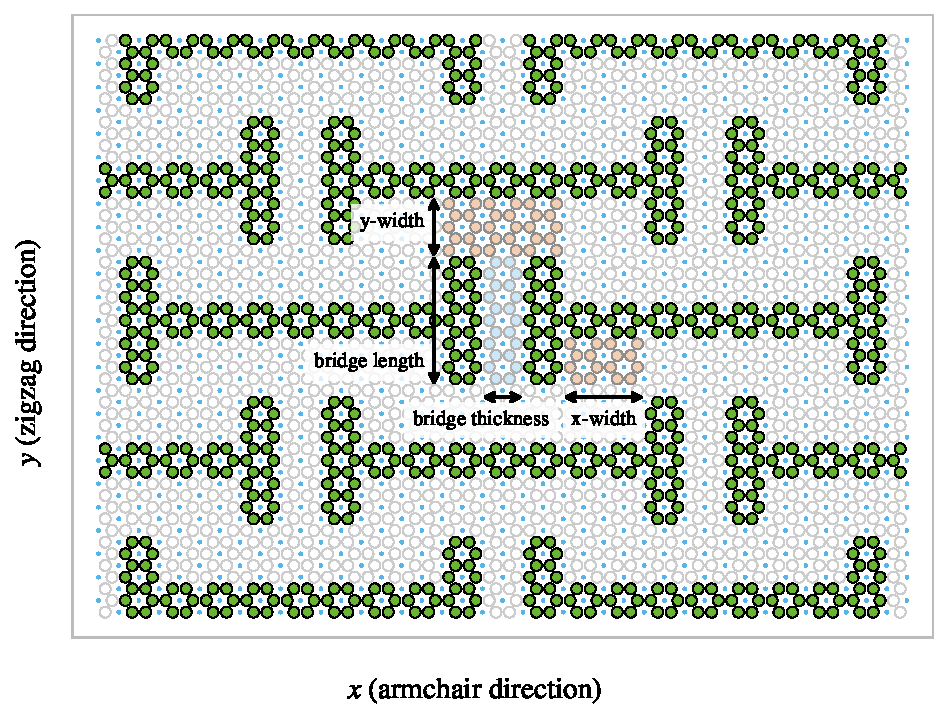
\includegraphics[width=\textwidth]{figures/system/honeycomb_inverse.pdf}
      \caption{}
      \label{fig:honeycomb_a}
    \end{subfigure}
    \hfill
    \begin{subfigure}[t]{0.48\textwidth}
      \centering
      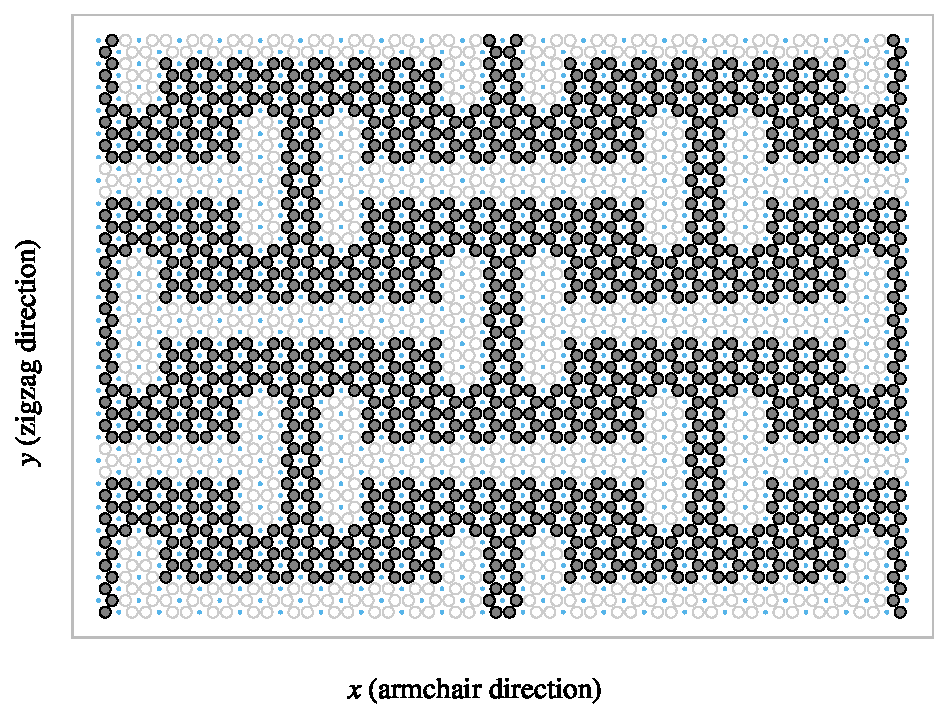
\includegraphics[width=\textwidth]{figures/system/honeycomb_pattern.pdf}
      \caption{}
      \label{fig:honeycomb_b}
  \end{subfigure}
  \hfill
     \caption{}
     \label{fig:honeycomb}
\end{figure}


\begin{figure}[H]
  \centering
  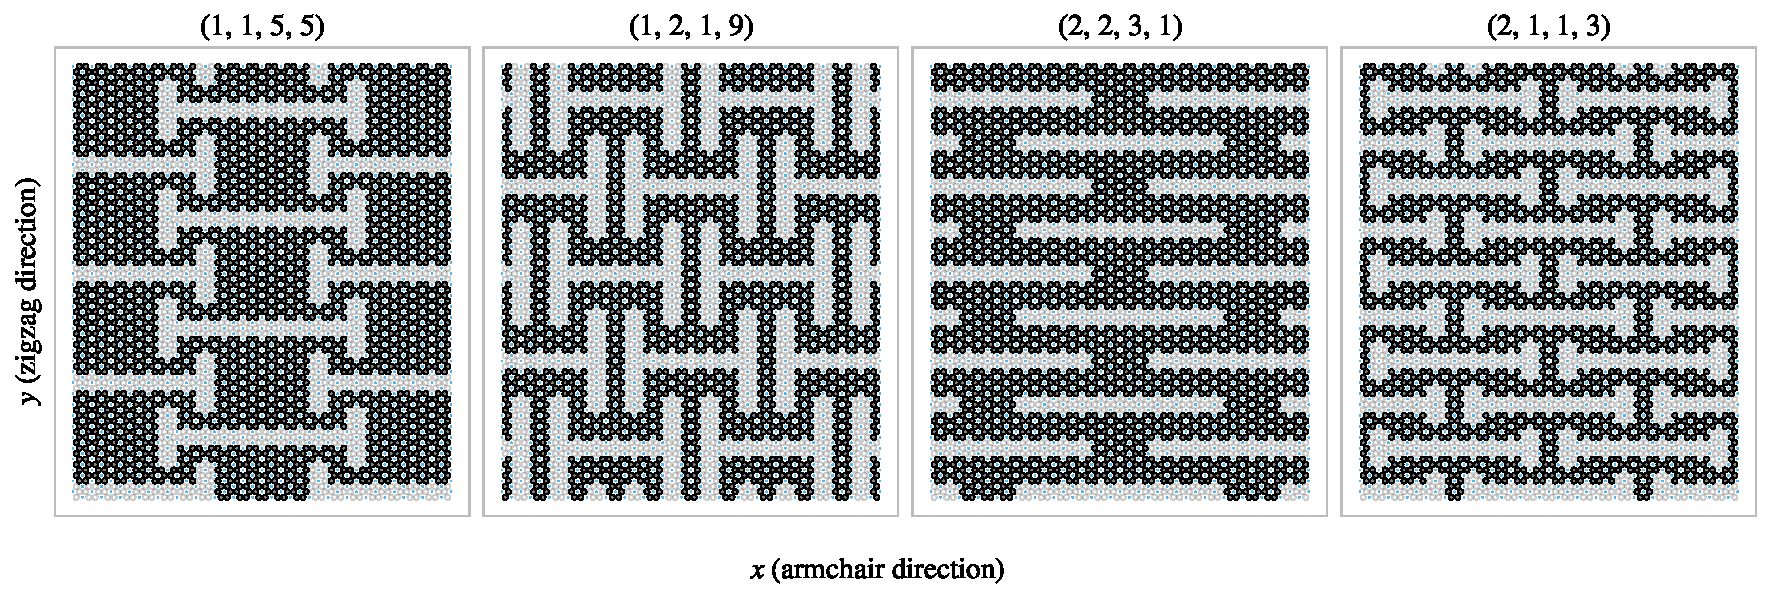
\includegraphics[width=\linewidth]{figures/system/honeycomb_flavors.pdf}
  \caption{}
  \label{fig:honeycomb_flavors}
\end{figure}




\subsection{Random walk}
The random walk serves as a method for introducing random patterns into the dataset with the scope of populating the configuration space more broadly than achieved purely with the more systematic patterns described above. By this argument, a straightforward way to create random configurations could be achieved simply by random noise, either uniform or gaussian. However, this would often leave the sheet detached with lots of non-connected atom clusters. Intuitively, we do not find this promising for the generation of large scale organized structures which we hypothesize to be of interest. The random walk pattern generation is characterized by the parameters summarized in \cref{tab:RW_params} which will be introduced throughout the following paragraphs. 

\begin{table}[H]
  \begin{center}
  \caption{Parameters for the random walk generator.}
  \label{tab:RW_params}
  \begin{tabular}{ | c | c | m{8cm} |} \hline
  \textbf{Parameters} & \textbf{Value} & \textbf{Description}  \\ \hline
  Num.\ walkers ($M$) & Integer $\ge$ 1 & Number of random walks to be initiated on the sheet (one at a time). \\ \hline
  Max.\ steps ($S$)  & Integer $\ge$ 1 &The maximum steps allowed for any random walker. \\ \hline
  Min.\ distance  & Integer $\ge$ 0 &The minimum distance required between any future paths and the previous paths in terms of the least walking steps in between. \\ \hline
  Bias  & Vector (direction, strength) & Bias direction and strength defining the discrete probability for the chocie of the next site. \\ \hline
  Connection  & Atoms / Center elements & Walk between atoms or between center elements (removing all adjecent atoms). \\ \hline
  Avoid unvalid  & True/False & Whether to remove already visited sites from the neighbour list before picking the next site. This prevents jumping to already visited site and lowers the likelihood of early termination.  \\ \hline
  Stay or break  & $p = [0,1]$ & \hl{Fill out} \\ \hline
  Periodic  & True/False & Whether to use periodic boundary conditions of all four sides. \\ \hline
  Avoid clustering  & Integer $\ge$ 0 & Amount of times to retry random walk in order to avoid detached clusters. Non-spanning clusters are removed after this amount of tries.\\ \hline
  RN6  & True/False & Randomly change the bias direction between one of the six center element directiosn for each random walker deployed. \\ \hline
  Grid start  & True/False & The option to have the random walkers start in an evenly spaced grid. \\ \hline
  Centering  & True/False & Relocate the path of a random walk after termination such that the path center of mass gets closer to the starting point (without violating the rules for travelling on already visited sites).\\ \hline
  \end{tabular}
  \end{center}
\end{table}

\subsubsection{Fundamentals} % M, S, Connection, Periodic, Avoid unvalid
For an uncut sheet we deploy $M$ random walkers, one at a time, and let them walk
for a maximum number of $S$ steps. We can either let the walker travel between
atom sites, removing the atoms in the path as it goes, or between center
elements, removing all sourrounding atoms --- \textit{Connection: Atom/Center
elements}. The method of removing only the intersecting atoms between center elements was also incorporated, but we ended up not using it due to plenty of other interesting options. Nonetheless, we will always remove a site once visited such that the
walker itself, or any other walkers, cannot use this site again. This corresponds
with the property of a self avoiding random walk, but it futhermore constraint
the walkers not to visit any path previously visited by others walkers which we might denote ``other avoiding'' then. By default, the walker has an equal chance of chosing any of its adjecent
neighbours for the next step, i.e.\ we draw the next step from a discrete
uniform distribution. Optionally we can use periodic bounary conditions,
\textit{Periodic: True/False}, allowing neighbouring sites to be connected
through the edge in both the x and y-direction. When traveling on atom sites
this ensures that we have three neighbour options for the next step while traveling on the
center elements this gives six neighbour options. If the walker happens to arrive at
an already visited site the walk is terminated early. Optionally, we can choose
to remove any neighbouring sites already visited from the neighbour list,
\textit{Avoid unvalid: True/False}, and choose uniformly between the remaining
options instead. This prolongs the walking distance, but the walker is
still able to find itself in a situation where no neighbouring sites are
availble, note that it cannot backtrack its own path either, and in such a case
the walk will be terminated dispite the setting of \textit{Avoid unvalid}.


\subsubsection{Spacing of walking paths} % minimum distance
In order to control the spacing between the paths of the various walkers we
implement a so-called, \textit{minimum distance: 0, 1, \ldots}, parameter
describing the spacing required between paths in terms of the least amount of
steps. When a walker has ended its walk, either by early termination or hitting
the maximum limits of steps, all sites within a walking distance of the minimum
distance is marked as visited, although they are not removed from the sheet.
This prevents any subsequent walkers to visit those sites in their walk
according to the general behaviour introduced in the previous paragraph. In
practice this is done through a recursive algorithm as described in algorithm
\cref{algo:walk_dis}. For a given path the function \textit{walk\_distance()} is called with the input being a list of all sites in the given paths. For each site, the function then gathers all site neighbours (regardless of their state on the sheet) and call itself using this neighbour list as input while incrementing a
distance counter passed along. This will result in an expansion along all
possible outgoing paths from the initial path of interest which is terminated
when the distance counter hits the distance limit. The function will
then return the final neighbour lists which is cummulated into a final output
corresponding to a list of all sites within the minimum distance to the path.

\begin{algorithm}[H]
  \caption{Recursive algorithm implemented as class method to mark sites within a distance of the class attribute self.min\_dis.}
  \label{algo:walk_dis}
  \begin{algorithmic}[1]
    \Require self.min\_dis $>$ 0 \Comment{This pseudocode does not handle other cases}
    \Function{walk\_distance}{self, input, dis = 0, pre = [ ]}
      % \State neigh $\gets$ NewList() 
      \State new\_neigh $\gets$ [ ] \Comment{Initialize list for new neighbours}
      \For{site in input}
        \State neigh $\gets$ get\_neighbouring\_sites(site) \Comment{Get sourrounding neighbours}
        \For{n in neigh}
          \If {(n not in pre) and (n not in new\_neigh)} \Comment{If not already added}
            \State AddItem(new\_neigh, n)
          \EndIf
        \EndFor
      \EndFor
      \State dis += 1 \Comment{Increment distance counter}
      \If{dis $\ge$ self.min\_dis} \Comment{Max limit hit}
        \State \Return input + new\_neigh 
      \Else \Comment{Start a new walk from each of the neighbouring sites}
        \State pre $\gets$ input
        \State \Return pre +  self.walk\_distance(new\_neigh, dis, pre)
      \EndIf
    \EndFunction
  \end{algorithmic}
\end{algorithm}

\hl{Do we need a figure supporting this?}

\subsubsection{Bias} % Bias
We include the option to perform biased random walk through the \text{Bias:
(direction, strength)} parameter option. We implement this by modelling each
walking step analog to the canonical ensemble under the influence of an
external force $\vec{F}$ representing the bias. For such a system each
microstate $i$, corresponding to the sites in the neighbour list, has the
associated probability $p_i$ given by the Gibbs–Boltzmann distribution
\begin{align*}
  p_{i} = \frac{1}{Z}e^{-\beta E_i}, \qquad Z = \sum_i e^{-\beta E_i},
\end{align*}
where $Z$ is the canonical partition function, $\beta = 1/k_B T$ for the
boltzmann constant $k_B$ and temperature $T$, and $E_i$ the energy of site $i$.
We model the energy of each site as the work required to move there. For a step
$\vec{s}$ the energy becomes $E_i = -\vec{s}\cdot\vec{F}$, where the sign is chosen such that the energy (difference) is negative when moving for aling the bias, analogous to an energy gain by
moving there. Due to the symmetry of both the atom sites and the center elements
sites the step length to neighbouring sites will always be equal. By defining
the bias magnitude $B = \beta|\vec{F}||\vec{s}|$ we the probability for
jumping to site $i$ as
\begin{align*}
  p_i = \frac{1}{Z}e^{B\hat{\vec{s}}\cdot\hat{\vec{F}}} \propto e^{B\hat{\vec{s}}\cdot\hat{\vec{F}}},
\end{align*}
 where the hat denotes the unit direction of the vector. The bias magnitude $B$ then captures the opposing effects of the magnitude of the external force and the
 temperature of the system as $B\propto |\vec{F}|/T$. We notice that
 $\hat{\vec{s}}\cdot\hat{\vec{F}} = \cos{(\theta)}$ for the angle $\theta$
 between the step and bias direction. This shows that the bias will have the
 biggest positive contribution to the probability when the step direction is fully allinged with the bias
 direction ($\theta = 0$), have no contribution for orthogonal directions
 ($\theta = \pm \pi/2$) and the biggest negative contribution when the directions
 are antiparallel ($\theta = \pi$). The partition function serves simply as a
 normalization constant. Thus, numerically we can enforce this simply by setting $Z = 1$ at first, calculate $p_i$, and then normalize the result at the final stage as a
 divition by the sum of all $p_i$. In the numerical implementation we then pick
 the step destination weighted by the discrete probability distribtion $p_i$. In
 \cref{fig:bias_prob} we have illustrated how a bias of different strength impacts the probability disitrbution for a random walk between center elements. We can visually confirm that the bias will favorise the directions that lies closes to the bias direction. This favorization is more distinct at high bias strengths while at low strength $B\to0$ we get a uniform distribution which alligns with the default unbiased random walk. 

\begin{figure}[H]
  \centering
  \begin{subfigure}[t]{0.48\textwidth}
      \centering
      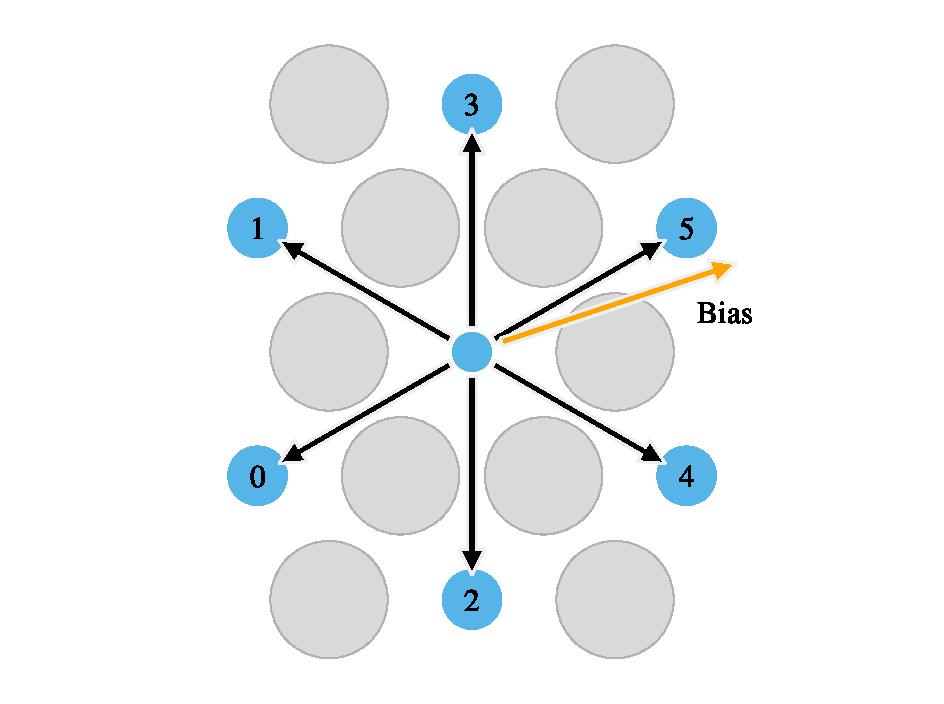
\includegraphics[width=\textwidth]{figures/system/bias_prob_a.pdf}
      \caption{}
      \label{fig:bias_prob_a}
    \end{subfigure}
    \hfill
    \begin{subfigure}[t]{0.48\textwidth}
      \centering
      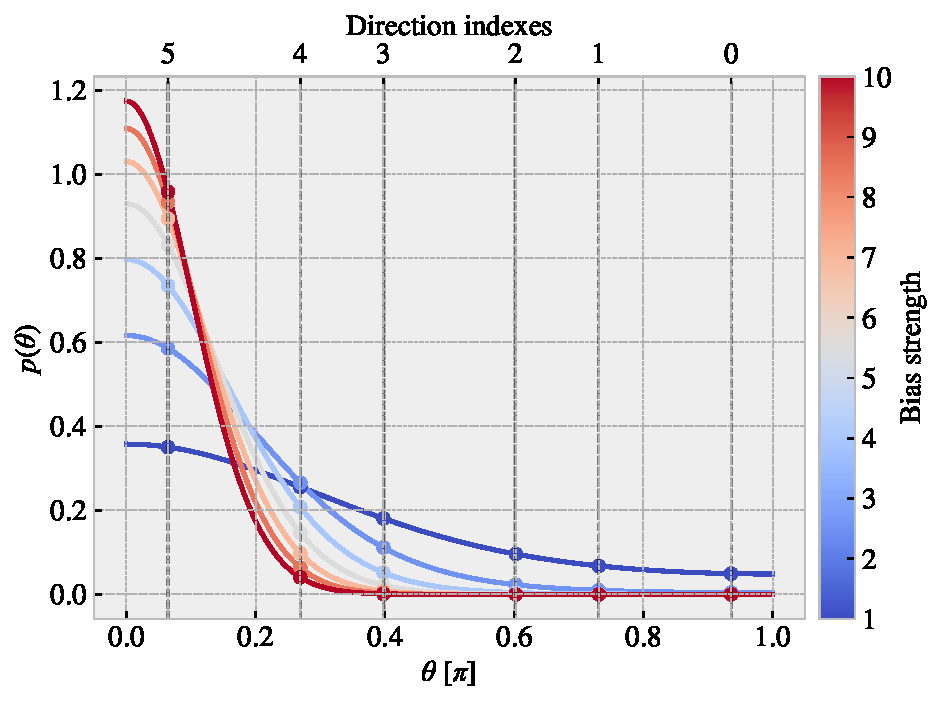
\includegraphics[width=\textwidth]{figures/system/bias_prob_b.pdf}
      \caption{}
      \label{fig:bias_prob_b}
  \end{subfigure}
  \hfill
     \caption{Illustration of the probability distribution for the various step direction during a bias random walked between center elements. $(a)$ Shows the possible step directions as black arrows pointing towards the neighbouring center elements shown as blue circles. The bias direction is denoted as an orange arrow and the numbering indicates the most likely direction to take (1) towards the least likely (6). The atoms sites are marked as grey circles for reference. $(b)$ The probability distribution as a function of angle between the direction of choice and the bias direction. The disitrbution is normalized according to the discrete probabilities marked with dots for which the continous line simple highlights the curve of the distribution. The direction indexes corresponds to the numbering on figure $(a)$. The color map indicates different strenghs of the bias. }
     \label{fig:bias_prob}
\end{figure}


\subsubsection{Stay or break}
The \textit{Stay or break: True/False} parameter defines the probability
$p_{\text{stay}}$ that the walker will keep its direction or otherwise break
into a different direction by probability $1-p_{\text{stay}}$. That is, we
manually substitute $p_{\text{stay}}$ in the discrete probability for the next
step corresponding to a continuation in the same direction. We then  shift the
remaining probabilities such that the distirbution remains normalized. In this
way we can still perform bias random walk in combination. For the center element
walk it is trivial to determine which of the neighbour directions correspond to
a continuation of direction based on the last visited site. However, for an atom site walk, it is not possible to follow the same direction in a straight line due to the hexagonal layout of the lattice. We recall that the
nearest atom neighbour indexes alternates for each increment in x or y index (see \cref{eq:atom_neigh_idx}) which corresponds to the alternating neighbour directions $D$
\begin{align*}
  (i + j) \ \text{is even} &\rightarrow D = \left\{ \frac{a}{2}\left(\frac{-2}{\sqrt{3}}, 0\right), \frac{a}{2}\left(\frac{1}{\sqrt{3}}, 1\right), \frac{a}{2}\left(\frac{1}{\sqrt{3}}, -1\right)\right\}, \\
  (i + j) \ \text{is odd} &\rightarrow D = \left\{ \frac{a}{2}\left(\frac{2}{\sqrt{3}}, 0\right), \frac{a}{2}\left(\frac{-1}{\sqrt{3}}, 1\right), \frac{a}{2}\left(\frac{-1}{\sqrt{3}}, -1\right)\right\}.
\end{align*}
One way to mittigate this issue is to use the six directions from the center element walk as the common direction to ``stay or break'' from. As showcased in \cref{fig:stay_or_break}, for each center element direction (black arrows) there are two possible atom directions (red and orange arrows) that are equally close to the center element direction. The red and orange arrows represent $(i+j)$ being even or odd respectively, and we notice that these appear in pairs such that we can always determine which of the atom directions that are closest to the center element direction. Following this idea we can map each center direction to an atom direction depending on the even or oddness of the position. For $p_{\text{stay}} = 1$ this results in a garuanteed zigzag motion along the center element direction that it happens to start on. 

\begin{figure}[H]
  \centering
  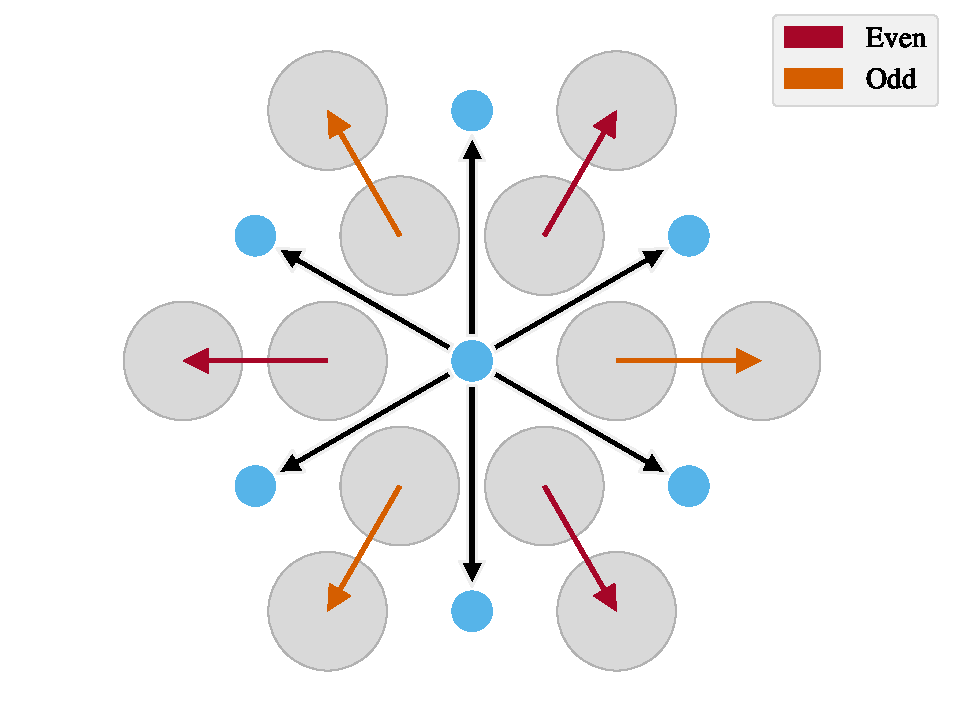
\includegraphics[width=0.5\linewidth]{figures/system/stay_or_break.pdf}
  \caption{\hl{Caption}}
  \label{fig:stay_or_break}
\end{figure}

The \textit{Stay or break} is still subject to previsouly defined rules, such that in the case that the site preferred site is not availble, it will either terminate when going there, or it is removed from the neighbour list when \textit{avoid unvalid: True}. For the latter case the walker has broken its direction and will follow the new direction with probability $p_{\text{stay}}$


\subsubsection{Deployment schemes} % Grid start, Centering, RN6
By default, each random walker is given an uniform random starting point among
the non-visited availble sites left on the sheet. This includes any modifications in relation to the minimum distance parameter. By toggling the \textit{Grid start:
True/False} parameter on, the starting points are instead predefined on an evenly
spaced grid. That is, the sheet is subdivided into the least amount of squares
that will accomodate a space for each starting point. 1 walker leads to a
$1\times 1$ partition, $\{2,3,4\}$ walkers lead to a $2\times 2$ partition,
$\{5,6,7,8,9\}$ walker lead to a $3\times 3$ partition and so on. For each partition square the starting point is placed as central as possible. The lower left partition square is then choosen as a default starting place for the first
walker and the remaining sites are filled according to the order that
maximizes the minimum distance between a new starting point and the ones already
used\footnote{In hindsight, it would have been less biased to choose a random partition square, but we do not consider this to be of great
importance for the usage of this feature in final dataset }. The population of the grid is visualized in \cref{fig:grid_start} for 1-9 walkers in total with color coding for the order of deployment. 


\begin{figure}[H]
  \centering
  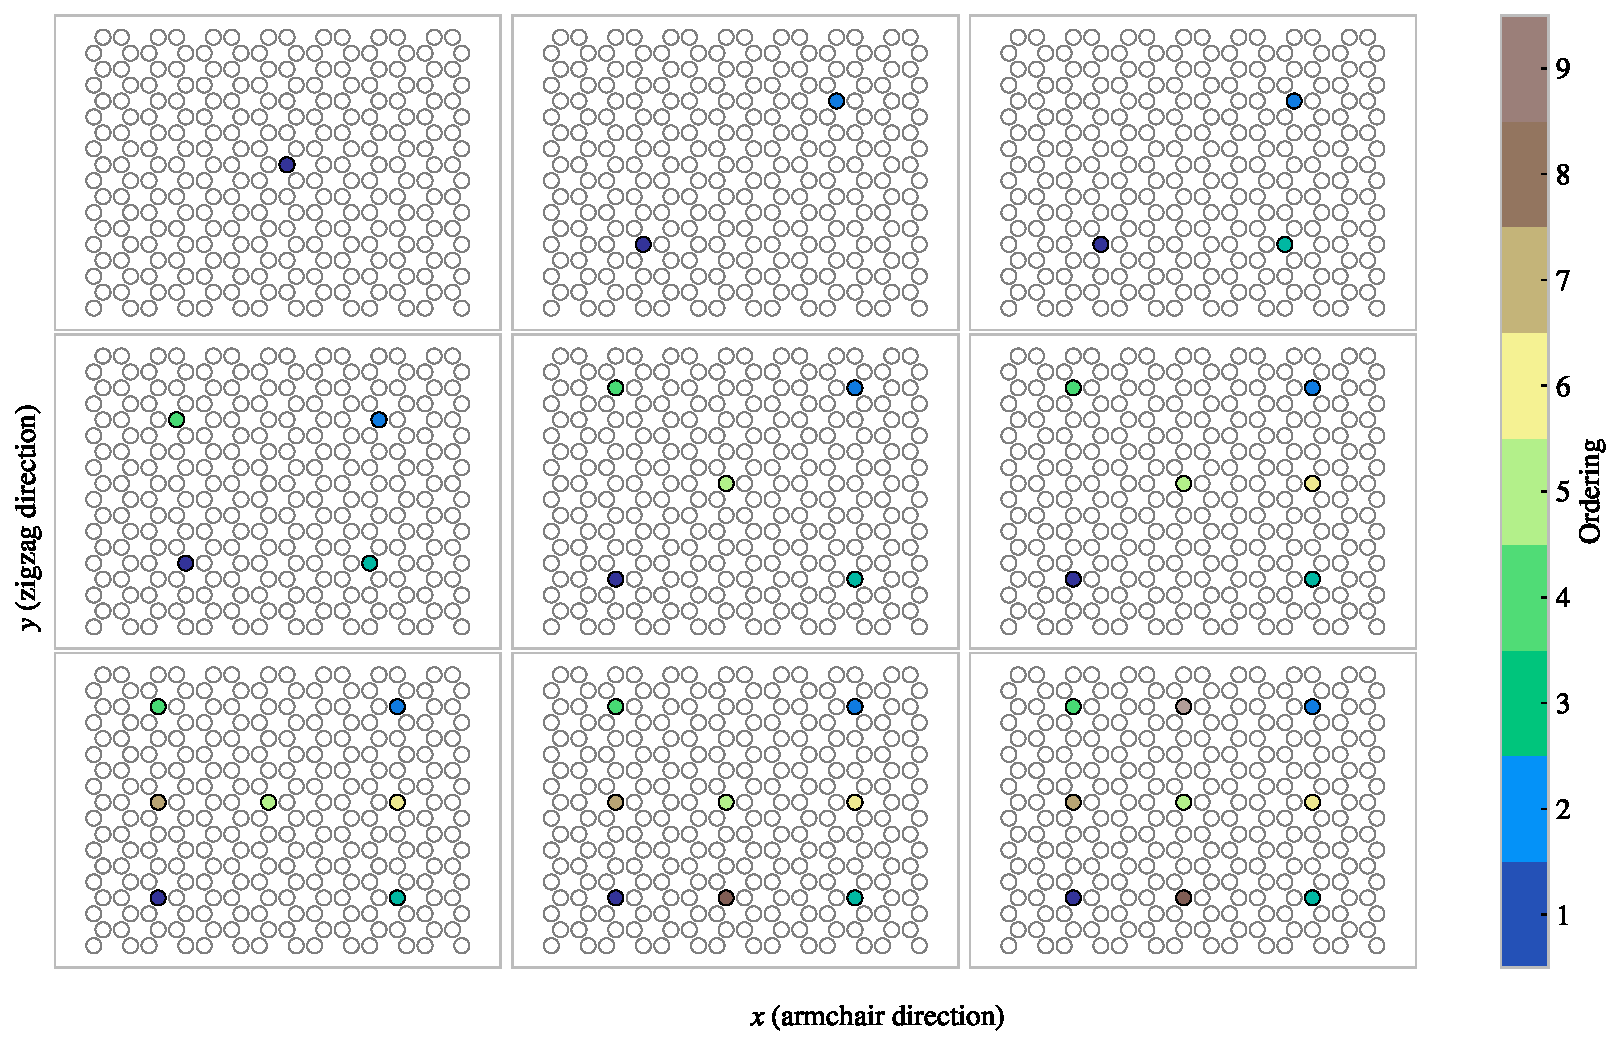
\includegraphics[width=\linewidth]{figures/system/grid_start.pdf}
  \caption{Populaiton of starting points with the centering parameter toggled on in a $14\times 18$ sheet. This is shown for 1-9 number of random walkers with the color map conveying the order of the population.}
  \label{fig:grid_start}
\end{figure}

The \textit{Centering: True/False} parameter let us relocate the path of the random walker such that the path center of mass alligns better with the starting point. When toggled on, the path is moved in the direction defined by the center of mass and the starting point for which the closest valid relocation on the direct translation line is choosen. This can be used in combination with the grid start and the bias parameter to make rather ordered configurations. In addition, the \textit{RN6:True/False} parameter can be used update the bias direction to on of the six directions of the center element walk for each new walker deplyoed. This lets us create confgiratiosn like the one shown in \cref{fig:RW_flavors}\textcolor{red!50!black}{b}. 


\subsubsection{Validity}
The simulation procedure requires the sheet to be fully attatched, non ruptured, which can be summarized as the following requirements. 
\begin{enumerate}
  \item There exist only a single cluster on the sheet. We define a cluster as the set of atoms which can all be reached through nearest neighbour walking on the cluster.
  \item The cluster of atoms is spanning the sheet in the y-direction. This means that there exist at least one path through nearest neighbour walks that connect the bottom and the top of the sheet. This is due to the reason that the sheet must be attatched to the pull blocks.
\end{enumerate}
In order to accommodate these requirements we count the number of clusters and search for a spanning cluster after all walkers have terminated. If the requirements are not met we simply rerun the random walk from scratch. This is done, \textit{Avoid clustering: 0, 1, \ldots}, amount of times. If the requirements are not met during any of those reruns the non-spanning clusters are simply removed. In the case of no spanning cluster the configuration is skipped. This crude scheme was later reinvented as a more refined repair scheme which alters the sheet by the intention of performing the least amount of changes (addition or subtraction of atoms) in order to meet the attatchment requirements. This was done as a part of the accelerated search procedure and hence it was not utilized in the creation of the random walk dataset. 

\subsubsection{Random walk examples}

Some examples of the random walk patterns are illustrated in \cref{fig:RW_flavors}.

\begin{figure}[H]
  \centering
  \includegraphics[width=\linewidth]{figures/system/RW_flavors.pdf}
  \caption{Some example uses of the random walking class. \hl{Give information of parameters?}}
  \label{fig:RW_flavors}
\end{figure}
